\documentclass[11pt]{amsart}
\usepackage[T1]{fontenc}
\usepackage{lmodern}
\input{glyphtounicode}
\pdfgentounicode=1
\usepackage{amsmath,amssymb}
\usepackage[table]{xcolor}
\usepackage{array}
\usepackage{booktabs}
\usepackage{longtable}
\usepackage{tikz}
\usepackage[margin=1in]{geometry}
\usepackage{url}
\usepackage[pdfauthor={311859884+mt0-svg@users.noreply.github.com},
            pdftitle={The frog model on the 4-ary tree is transient},
            pdfkeywords={frog model, interacting random walks, d-ary tree, transience, recurrence, stochastic domination, recursive distributional inequality, certificate, Lean 4, formal verification},
            bookmarksnumbered=true]{hyperref}
\hypersetup{colorlinks=true, linkcolor=blue, citecolor=blue, urlcolor=blue}
\makeatletter\g@addto@macro\UrlBreaks{\do\.\do\_}\makeatother
\Urlmuskip=0mu plus 1mu
\emergencystretch=3em
\newcommand{\repo}{https://github.com/mt0-svg/frog-model-tree}
% robust, so that amsart does not uppercase the address in the author line
\DeclareRobustCommand{\authorlink}{\href{\repo/issues/new/choose}{\nolinkurl{311859884+mt0-svg@users.noreply.github.com}}}

\newtheorem{theorem}{Theorem}[section]
\newtheorem{lemma}[theorem]{Lemma}
\newtheorem{proposition}[theorem]{Proposition}
\newtheorem{corollary}[theorem]{Corollary}
\newtheorem{conjecture}[theorem]{Conjecture}
\theoremstyle{definition}
\newtheorem{definition}[theorem]{Definition}
\newtheorem{remark}[theorem]{Remark}
\numberwithin{equation}{section}

% The map from the paper to the checks, next to each \label; these two macros print nothing.
% paper/statement_map.sh reads them and writes STATEMENTS.md.
%   \lean{A, B, ...}      the Lean declarations of the statement, the first being the one its proof names;
%   \computed{p, q, ...}  scripts and recorded outputs, paths from the root of the repository;
%   \nolean{reason}       for a statement with no Lean declaration, the reason.
\newcommand{\lean}[1]{\ignorespaces}
\newcommand{\computed}[1]{\ignorespaces}
\newcommand{\nolean}[1]{\ignorespaces}
% the Lean declaration named in the last sentence of a proof
\DeclareUrlCommand\decl{\urlstyle{tt}}

\newcommand{\T}{\mathbb{T}}
\newcommand{\Ts}{\mathbb{T}^{*}}
\newcommand{\N}{\mathbb{N}}
\newcommand{\Nb}{\overline{\mathbb{N}}}
\newcommand{\E}{\mathbf{E}}
\renewcommand{\P}{\mathbf{P}}
\newcommand{\cst}{\gamma}
\newcommand{\BR}{\operatorname{BR}}
\newcommand{\cS}{\mathcal{S}}
\newcommand{\cA}{\mathcal{A}}
\newcommand{\cC}{\mathcal{C}}
\newcommand{\cU}{\mathcal{U}}
\newcommand{\cW}{\mathcal{W}}
\newcommand{\eps}{\varepsilon}
\newcommand{\stle}{\preceq}
\newcommand{\one}{\mathbf{1}}

\begin{document}

\title[The frog model on the 4-ary tree]{The frog model on the 4-ary tree is transient}
\author{\authorlink}
\thanks{2020 {\em Mathematics Subject Classification.} Primary: 60K35; Secondary: 60J80, 60J10, 60E15, 03B35.\\\indent
{\em Key words and phrases.} Frog model; interacting random walks; $d$-ary tree; transience; stochastic domination; recursive distributional inequality; certificate; Lean~4.}

\begin{abstract}
We prove that the frog model on the rooted $4$-ary tree is transient. One frog starts awake at the root and one sleeps at every other vertex; awake frogs perform independent simple random walks, waking the frogs they visit. Almost surely the root is visited finitely often; the mean number of visits is at most $5.756$. This is the case $d=4$ of a conjecture of Hoffman, Johnson and Junge on the $d$-ary tree, who proved recurrence for $d=2$ and transience for $d\ge5$. The proof bounds by $0.536$ the mean number of frogs that a subtree sends back to the parent of its root. It combines an exact recursion on the laws of the response curves of subtrees with a law, given by a finite table, that dominates its image; two linear systems on $159786$ states certify the domination. The proof is formalized in Lean~4, whose kernel checks the certificate.
\end{abstract}

\maketitle

\definecolor{leangreen}{RGB}{0,122,61}
\newcommand{\badge}[2]{\colorbox{#1}{\strut\textcolor{white}{\sffamily\bfseries\small #2}}}
\begin{center}
\small
\renewcommand{\arraystretch}{1.5}
\begin{tabular}{>{\raggedright\arraybackslash}p{0.2\textwidth} >{\raggedright\arraybackslash}p{0.7\textwidth}}
\rowcolor{black!6}
\multicolumn{2}{>{\raggedright\arraybackslash}p{0.93\textwidth}}{\textit{This is AI-generated research: the results, proofs and code were found and written by AI. Credit goes to all the humans whose work it builds on.}}\\
\badge{leangreen}{Proved in Lean 4} & Theorem~\ref{thm:main} is proved in Lean~4 with Mathlib, with no hypothesis and only the standard axioms (\texttt{FrogModel.transient\_four} and \texttt{FrogModel.meanVisits\_four\_le}). So are Theorems~\ref{thm:A} and~\ref{thm:B} and the numbered statements of Sections~\ref{sec:thmA} to~\ref{sec:certificate}, those of Section~\ref{sec:criterion} for the table of Section~\ref{sec:certificate}, and the Lean kernel checks the certificate of Section~\ref{sec:certificate}. Comparator checks the two theorems against a copy of their statements, and nanoda, a second implementation of the Lean kernel, checks them again.\\
\rowcolor{black!6}
\multicolumn{2}{>{\raggedright\arraybackslash}p{0.93\textwidth}}{Lean proofs, code, certificates and the \TeX{} source: \href{\repo}{\texttt{github.com/mt0-svg/frog-model-tree}}}\\
\end{tabular}
\end{center}

\clearpage
\section{Introduction}\label{sec:intro}

We prove that the frog model on the rooted $4$-ary tree is transient: the root is visited only finitely many times, almost surely. This is the case $d=4$ of a conjecture of Hoffman, Johnson and Junge \cite{HJJ17}. The proof reduces the question to a bound on the mean number of frogs that a subtree sends back through its top edge, and proves that bound with a finite certificate.

The frog model on the rooted $d$-ary tree $\T_d$ is the following system of random walks.
\begin{enumerate}
\item The vertices of $\T_d$ are the finite words over the alphabet $\{1,\dots,d\}$; the root is the empty word $\varnothing$, and the children of a vertex $v$ are the words $v1,\dots,vd$. So the root has degree $d$ and every other vertex has degree $d+1$.
\item At every vertex $v$ sits one frog $f_v$, with a path $(S_v(n))_{n\ge0}$, a simple random walk on $\T_d$ started at $v$; the paths of the frogs are independent.
\item At time $0$ the frog $f_\varnothing$ is awake and every other frog is asleep. A sleeping frog wakes at the first time an awake frog is at its vertex, and a frog woken at time $s$ is at $S_v(t-s)$ at every time $t\ge s$.
\end{enumerate}
The quantity of interest is the number of visits to the root after time $0$,
\begin{equation}\label{eq:V}
V=\#\{(v,t):\ t\ge1,\ f_v \text{ is awake at time } t \text{ and } S_v(t-s_v)=\varnothing\},
\end{equation}
where $s_v$ is the time at which $f_v$ wakes. The model is \emph{transient} if $V<\infty$ almost surely and \emph{recurrent} if $V=\infty$ almost surely.

Popov asked whether the model with one frog per vertex is recurrent on the tree in which every vertex has degree $d$ \cite[Open Problem~4.1]{Pop03}. Hoffman, Johnson and Junge proved that the frog model on $\T_2$ is recurrent and that the frog model on $\T_d$ is transient for every $d\ge5$ \cite[Theorem~1]{HJJ17}, and they left the two remaining degrees as a conjecture.

\begin{conjecture}[{Hoffman, Johnson and Junge \cite[Conjecture~2, p.~2828]{HJJ17}}]\label{conj:HJJ}\nolean{a quoted conjecture, whose case d = 4 is the main theorem}
The frog model on $\T_d$ is recurrent a.s. for $d = 3$ and transient a.s. for $d = 4$.
\end{conjecture}

\begin{theorem}\label{thm:main}\lean{FrogModel.transient_four, FrogModel.meanVisits_four_le, FrogModel.Transient, FrogModel.transient_four_of_data, FrogModel.meanVisits_four_le_of_data, FrogModel.meanVisits_four_le_exact_of_data}\computed{code/gp/small_checks.gp, code/gp/small_checks.out}
For $d=4$, $V<\infty$ almost surely, and $\E V\le5.756$.
\end{theorem}

So the second half of Conjecture~\ref{conj:HJJ} holds; the first half, recurrence for $d=3$, remains open.

\subsection*{What was known}
For $d\ge5$ Hoffman, Johnson and Junge compare the projection of the frog model on the distance to the root with a branching random walk. For $d\ge6$ one type suffices, and a normalized exponential weight of the configuration is a martingale \cite[Proposition~18]{HJJ17}; for $d=5$ the walk has $27$ types, whose transition probabilities are computed with computer assistance. The same method, with $6$ types, gives transience on the tree whose levels alternate between $5$ and $6$ children \cite[Proposition~19]{HJJ17}. They write that ``conceptually our approach could extend to a computer-assisted proof for transience when $d = 4$, but the demands of this theoretical program seem well beyond current processing power'' \cite[p.~2829]{HJJ17}. Their Conjecture~2 rests on simulations of the model with stunning fences \cite[Section~5]{HJJ17}: a frog that reaches depth $k$ stops there until all frogs have stopped, and the growth in $k$ of the number $A_{d,k}$ of frogs that pile up at depth $k$ suggests recurrence for $d=3$ and transience for $d=4$. This staged picture is the nearest precursor of steps~2 to~5 of the method below. With independent Poisson numbers of frogs of mean $\mu$ per vertex, the model is transient when $\mu<(d-1)^2/(4d)$ \cite[Proposition~15]{HJJ16}, which is $9/16$ for $d=4$, and the critical density lies between $0.24d$ and $2.28d$ for large $d$ \cite[Theorem~1]{JJ16}. Johnson and Junge extend transience for $d\ge5$ to every configuration of mean at most one per vertex by stochastic orders \cite[Corollary~7]{JJ18}, while for every $\mu$ some law of mean $\mu$ for the initial numbers of frogs makes the model on $\T_d$ transient \cite[Theorem~1.1]{JR19}. Rosenberg proves recurrence on the tree whose levels alternate between $3$ and $2$ children \cite[Theorem~1.1]{Ros18}. In their study of the cover time, Hoffman, Johnson and Junge plant the $d$-ary tree of height $H$ below an extra vertex $y$ and freeze the frogs that reach $y$ \cite[Proposition~4.3]{HJJ19}, and in the proof of \cite[Corollary~4.4]{HJJ19} they sort the frogs that return to the root up to a time $2^j$ into generations, the mean of each generation at most $1+\mu$ times the mean frozen count times the mean of the previous one, with $\mu$ the mean number of sleeping frogs per vertex. Theorem~\ref{thm:A} runs this argument for all time and charges the frogs of the children of the root once in all instead of once per generation (Lemma~\ref{lem:children}), which turns the condition $2x_d<1$ of one frog per vertex into $x_d<1$; this matters here, since the bound of Theorem~\ref{thm:B} exceeds $1/2$. On $\mathbb{Z}^2$ with drift, D\"obler, Gantert, H\"ofelsauer, Popov and Weidner stop the frogs at hyperplanes and refill, before each particle branches, every vertex whose frog has woken, which gives a branching random walk with independent offspring that visits every vertex the frog model visits \cite[proof of Theorem~1.1(ii)]{DGHPW18}; Lemma~\ref{lem:refresh} plays the same role in the proof of Theorem~\ref{thm:A}, where it charges each excursion with an independent copy of the frozen count. The cases $d=3$ and $d=4$ are stated as open in \cite{JJ16,BFJJT19,MR24,MW20,AJ25,Fra26}, and simulations of the model with $d=4$ point to transience \cite[Section~5]{HJJ17}. Related work treats the frog model with drift on $\T_d$ \cite{BFJJT19,GTW22,BJL24,Mat24}, on Galton-Watson trees \cite{MR24,MW20} and on non-amenable trees \cite{MR20}, the cover time and the susceptibility on finite $d$-ary trees \cite{HJJ19,Her18}, and frogs with geometric lifetimes on trees \cite{GR18,Pen24}.

\subsection*{The method}
Freeze at $y$ the frogs of a planted copy of $\T_4$ and let $x_4$ be the mean number of frozen frogs (Definition~\ref{def:planted}). The proof has five steps.
\begin{enumerate}
\item The bound $\E V\le(d+1)x_d/(1-x_d)$ whenever $x_d<1$ (Theorem~\ref{thm:A}, Section~\ref{sec:thmA}). The visits to the root are sorted into generations of excursions from the root, and each excursion into a subtree is charged with an independent copy of the frozen count.
\item The frozen count is the first value of a random response curve, the number of frozen frogs as a function of the number of frogs started at the root, and the law of the response curve of the tree truncated at depth $K$ is the image of the law at depth $K-1$ under an explicit map $\Psi$ (Lemma~\ref{lem:recursion}, Section~\ref{sec:curves}). The map is monotone for the stochastic order.
\item The response curve is dominated by a curve made of independent blocks of $J$ values, each with the law of the first $J$ values of the curve itself (Proposition~\ref{prop:renewal}, Section~\ref{sec:renewal}). So every law $H^*$ of blocks of $J$ values that dominates its own image under the induced map $\Phi_J$ bounds $x_d$ by the mean of its first coordinate (Theorem~\ref{thm:super}).
\item For $d=4$ and a law $H^*$ given by a finite table, the image $\Phi_4(H^*)$ is the output law of a Markov chain on states made of the four children and the frogs waiting at the root. A potential bounds the exponential moments of its output, replacing a child by a dominating one can only raise the output, and finitely many inequalities, on the table and on two linear systems over a finite set of states, imply $\Phi_4(H^*)\stle H^*$ (Theorem~\ref{thm:check}, Section~\ref{sec:criterion}).
\item A table with $31$ rows and data on $159786$ states satisfy these inequalities, with $\E B^*(1)=\cst=0.53513682\ldots$ (Proposition~\ref{prop:cert}, Section~\ref{sec:certificate}). So $x_4\le\cst$, and $\E V\le5\cst/(1-\cst)<5.756$.
\end{enumerate}
The bound needed, $x_4<1$, holds with room, since the table law has mean $0.535$. What makes a finite table enough is that the recursion of step~2 keeps the dependence between the frogs returned by one subtree: the response curve records how many frogs come back for every number of frogs sent in, and blocks of four values of it already suffice in step~5.

\subsection*{The formalization}
Theorem~\ref{thm:main} is proved in Lean~4 with Mathlib, with no hypothesis and only the standard axioms, from the definition of the model given above. So are Theorems~\ref{thm:A} and~\ref{thm:B} and the numbered statements of Sections~\ref{sec:thmA} to~\ref{sec:certificate}; those of Section~\ref{sec:criterion} are proved for the table of Section~\ref{sec:certificate}, the one the proof uses. The finite verifications of Section~\ref{sec:certificate} are evaluations in the Lean kernel, and no compiled code is trusted. Each formalized proof ends with the name of its main Lean declaration. Section~\ref{sec:comp} describes the formal proof and its data, and the repository lists, for every numbered statement, the declarations of its formal proof.

Section~\ref{sec:reduction} proves Theorem~\ref{thm:main} from Theorems~\ref{thm:A} and~\ref{thm:B}, Sections~\ref{sec:thmA} to~\ref{sec:certificate} prove them, Section~\ref{sec:comp} describes the formal proof and its data, and Appendix~\ref{app:table} lists the table.

\section{Frozen frogs}\label{sec:reduction}

This section reduces Theorem~\ref{thm:main} to two statements about one planted subtree. Theorem~\ref{thm:A} bounds the expected number of visits to the root by the mean number of frogs that a planted subtree sends to the parent of its root, and Theorem~\ref{thm:B} bounds this mean when $d=4$. Throughout, $d\ge2$, $\Nb=\{0,1,2,\dots\}\cup\{\infty\}$, and $\T(v)$ is the subtree of $\T_d$ made of $v$ and its descendants.

\begin{definition}[the planted tree]\label{def:planted}
The planted tree $\Ts$ is $\T_d$ with one more vertex $y$, joined to the root of $\T_d$ only; we write $r$ for that root, so that $r$ has degree $d+1$ in $\Ts$ and $y$ is a leaf. The frog model on $\Ts$ has one awake frog at $r$, no frog at $y$ and one sleeping frog at every other vertex. The frogs follow independent simple random walks on $\Ts$, and a frog stops for good at its first visit to $y$: it is \emph{frozen}. Let $X\in\Nb$ be the number of frogs that are woken and frozen, and $x_d=\E X$.
\end{definition}

\begin{figure}[ht]
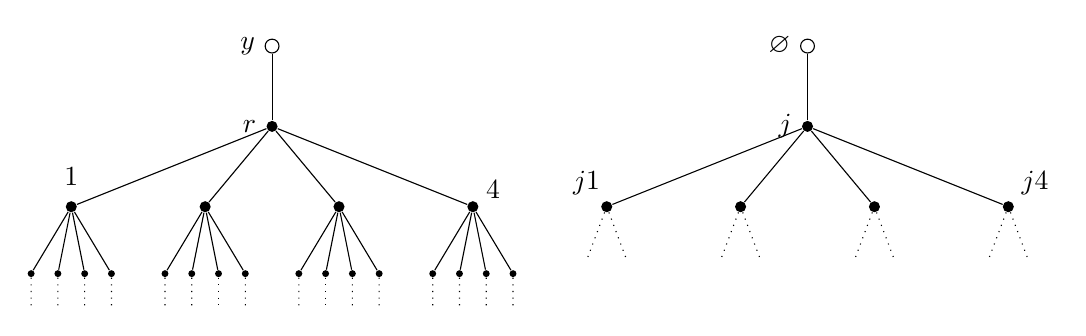
\begin{tikzpicture}[scale=0.85,
  v/.style={circle,fill,inner sep=0,minimum size=4pt},
  e/.style={circle,draw,inner sep=0,minimum size=5pt}]
\node[e,label=left:{$y$}] (y) at (0,1.2) {};
\node[v,label=left:{$r$}] (r) at (0,0) {};
\draw (y)--(r);
\foreach \i/\x in {1/-3,2/-1,3/1,4/3} {
  \node[v] (c\i) at (\x,-1.2) {};
  \draw (r)--(c\i);
  \foreach \k/\dx in {1/-0.6,2/-0.2,3/0.2,4/0.6} {
    \node[v,minimum size=2.5pt] (g\i\k) at (\x+\dx,-2.2) {};
    \draw (c\i)--(g\i\k);
    \draw[dotted] (g\i\k)--++(0,-0.5);
  }
}
\node at (-3,-0.75) {$1$};
\node at (3.3,-0.95) {$4$};
\begin{scope}[xshift=8cm]
\node[e,label=left:{$\varnothing$}] (o) at (0,1.2) {};
\node[v,label=left:{$j$}] (j) at (0,0) {};
\draw (o)--(j);
\foreach \k/\x in {1/-3,2/-1,3/1,4/3} {
  \node[v] (h\k) at (\x,-1.2) {};
  \draw (j)--(h\k);
  \draw[dotted] (h\k)--++(-0.3,-0.8);
  \draw[dotted] (h\k)--++(0.3,-0.8);
}
\node at (-3.3,-0.85) {$j1$};
\node at (3.4,-0.85) {$j4$};
\end{scope}
\end{tikzpicture}
\caption{The planted tree $\Ts$ for $d=4$ (left), and the subtree $\T(j)$ of a child $j$ of the root of $\T_4$ with the root $\varnothing$ above it (right). The second graph is the first one with $r=j$ and $y=\varnothing$.}\label{fig:planted}
\end{figure}

For a child $j$ of the root of $\T_d$, the graph $\T(j)\cup\{\varnothing\}$ is a copy of $\Ts$ in which $j$ plays the role of $r$ and $\varnothing$ that of $y$ (Figure~\ref{fig:planted}). Every vertex of $\T(j)$ has degree $d+1$ both in $\T_d$ and in this copy, so a simple random walk on $\T_d$ from a vertex of $\T(j)$, stopped at its first visit to $\varnothing$, is a simple random walk on $\Ts$ stopped at $y$. This is how $X$ enters: the frogs that leave a subtree of the root through its top edge are the frozen frogs of a planted tree.

\begin{theorem}\label{thm:A}\lean{FrogModel.theoremA, FrogModel.transient_of_meanX_lt_one, FrogModel.meanX, FrogModel.frozenCount}
Let $d\ge2$ and suppose that $x_d<1$. Then
\[
\E V\le \frac{(d+1)\,x_d}{1-x_d},
\]
and the frog model on $\T_d$ is transient.
\end{theorem}

Each return of a frog to the root starts an excursion into one of the $d$ subtrees of the root, which can wake frogs there and send some of them back to the root; Theorem~\ref{thm:A} charges each such excursion with an independent copy of $X$. The numerator $(d+1)x_d$ bounds the expected number of returns caused by the frog of the root and by the frogs of the $d$ children of the root, each counted once, and the factor $1/(1-x_d)$ sums the returns of later generations. The freezing at $y$ is what makes this an upper bound: a frog frozen at $y$ is a return to the root of $\T_d$, and everything it does afterwards is charged to the next generation.

\begin{theorem}\label{thm:B}\lean{FrogModel.lemmaXFour_of_data, FrogModel.LemmaX.lemmaXFour_of, FrogModel.LemmaX.LemmaXFour, FrogModel.LemmaX.meanHstar_holds}
For $d=4$,
\[
x_4\le\cst,\qquad \cst=\frac{9337230319347}{17448304640000}=0.53513682\ldots
\]
\end{theorem}

\begin{proof}[Proof of Theorem~\ref{thm:main}]
By Theorem~\ref{thm:B}, $x_4\le\cst<1$, so Theorem~\ref{thm:A} applies with $d=4$. Since $t\mapsto t/(1-t)$ is increasing on $[0,1)$, it gives
\[
\E V\le\frac{5x_4}{1-x_4}\le\frac{5\cst}{1-\cst}=\frac{46686151596735}{8111074320653}=5.7558530\ldots<5.756,
\]
and in particular $V<\infty$ almost surely. This is \decl{FrogModel.transient_four} in the formalization, with \texttt{FrogModel.meanVisits\_four\_le} for the bound on $\E V$.
\end{proof}

The proof of Theorem~\ref{thm:B} occupies Sections~\ref{sec:curves} to~\ref{sec:certificate}. Section~\ref{sec:curves} writes the number of frozen frogs of $\Ts$ as the first value of a random response curve, whose law satisfies an exact recursion through the subtrees of the children of $r$. Section~\ref{sec:renewal} shows that a law $H^*$ of blocks of response values that dominates its own image under the recursion bounds $x_4$ by the mean of its first coordinate. Section~\ref{sec:criterion} turns the domination of a law given by a finite table into finitely many inequalities, and Section~\ref{sec:certificate} gives the table and checks the inequalities.

\section{Proof of Theorem~\ref{thm:A}}\label{sec:thmA}

This section proves Theorem~\ref{thm:A}, by the argument of the proof of \cite[Corollary~4.4]{HJJ19} run for all time. The visits to the root are sorted into generations, called stages: the frog of the root forms stage $1$, and an excursion from the root that starts at the end of an excursion of stage $i$ belongs to stage $i+1$, together with everything it wakes. Lemma~\ref{lem:visits} bounds $V$ by the number of excursions of all stages, and Lemma~\ref{lem:stage} bounds the expected number of excursions of stage $i+1$ by $x_d$ times the expected number of excursions of stage $i$ plus a correction, whose total Lemma~\ref{lem:children} bounds by $d$. The independence that Lemma~\ref{lem:stage} needs comes from Lemma~\ref{lem:refresh}.

\subsection{Reachability}\label{sec:reach}
The set of frogs that wake does not depend on the times at which the frogs move, only on their paths. Lemma~\ref{lem:reach}, used throughout the paper, says so.

\begin{lemma}\label{lem:reach}\lean{FrogModel.woken_iff_reach, FrogModel.encard_visits}
Consider the frog model on $\T_d$ with given paths $S_v$, $S_v(0)=v$. Let $D$ be the directed graph on the frogs with an arc $f_u\to f_w$ whenever $w\neq\varnothing$ and $w=S_u(n)$ for some $n\ge0$. Then a frog is ever woken if and only if it is reachable from $f_\varnothing$ in $D$, and
\[
V=\#\{(v,n):\ f_v \text{ is reachable from } f_\varnothing,\ n\ge1,\ S_v(n)=\varnothing\}.
\]
\end{lemma}

The same holds on $\Ts$, with arcs to the vertices other than $r$ and $y$ and with the stopped paths. There we take it as the definition of the number of frozen frogs: $X$ is the number of frogs reachable from the frog at $r$ whose path visits $y$.

\begin{proof}
If $f_u$ is woken and $f_u\to f_w$, then $f_u$ is at $w$ at some time, so $f_w$ is woken by then; by induction along a path of $D$, every frog reachable from $f_\varnothing$ is woken. Conversely, by induction on the time at which it wakes, a frog woken at a time $t>0$ was woken by an awake frog $f_u$ at its vertex at time $t$, so $f_u\to f_w$ with $f_u$ woken before $t$. A pair $(v,t)$ counted in~\eqref{eq:V} is mapped to $(v,t-s_v)$, injectively, and the image is the set on the right. This is \decl{FrogModel.woken_iff_reach} in the formalization, for the first claim.
\end{proof}

\subsection{Pieces, segments and stages}\label{sec:stages}
The paths of the frogs are cut at their visits to the root. A \emph{segment} is a pair $\sigma=(u,k)$ of a vertex $u$ and an integer $k\ge0$. To each segment we attach a \emph{piece} $\omega_\sigma=(\omega_\sigma(n))_{n\ge0}$, a simple random walk on $\T_d$ started at $u$ if $k=0$ and at $\varnothing$ if $k\ge1$, all pieces independent. The \emph{cut} of a piece is $\tau_\sigma=\min\{n\ge1:\omega_\sigma(n)=\varnothing\}\in\Nb$, and $\sigma$ is \emph{closed} when $\tau_\sigma<\infty$. The \emph{glued path} $S_u$ follows $\omega_{(u,0)}$ up to its cut, then $\omega_{(u,1)}$ up to its cut, and so on, up to the first piece with an infinite cut.

The proof of Theorem~\ref{thm:A} builds the frog model from the pieces, which Lemma~\ref{lem:glue} allows.

\begin{lemma}\label{lem:glue}\lean{FrogModel.map_glue, FrogModel.lintegral_visits_eq}
The glued paths $(S_u)_u$ are independent simple random walks on $\T_d$, $S_u$ started at $u$.
\end{lemma}

\begin{proof}
By the strong Markov property of simple random walk at its successive visits to $\varnothing$, a simple random walk from $u$ is the concatenation of independent pieces with these laws, cut at their returns to $\varnothing$. The pieces of different frogs are independent. This is \decl{FrogModel.map_glue} in the formalization.
\end{proof}

So the frog model may be built from the pieces, and we do so in the rest of this section. Two kinds of arcs join segments. A segment $\sigma$ \emph{wakes} the segment $(w,0)$ when $w\neq\varnothing$ and $\omega_\sigma(n)=w$ for some $n\le\tau_\sigma$; the \emph{successor} of a closed segment $(u,k)$ is $(u,k+1)$. For a set $B$ of segments, its \emph{closure} is the smallest set of segments that contains $B$ and contains every segment woken by one of its members. The stages are
\[
\cS_0=\emptyset,\qquad \cS_{i+1}=\text{the closure of } B_i,\qquad B_i=\{(\varnothing,0)\}\cup\cS_i\cup\{(u,k+1):(u,k)\in\cS_i \text{ closed}\},
\]
and the segments that enter at stage $i+1$ are $Z_i=B_i\setminus\cS_i$, of number $R_i=|Z_i|\in\Nb$. So $Z_0=\{(\varnothing,0)\}$, $R_0=1$, and for $i\ge1$ every segment of $Z_i$ is the successor of a closed segment of $\cS_i$, a piece that starts at the root. The stages increase with~$i$.

A piece that starts at the root steps first to a child $j$ of the root, and stays in $\T(j)$ until its cut; a piece $\omega_{(w,0)}$ with $w\in\T(j)$ stays in $\T(j)$ until its cut. For a child $j$ of the root, let $Z_i(j)$ be the set of segments of $Z_i$ whose piece steps first to $j$, and
\[
\cA_j=\begin{cases}Z_i(j)\cup\{(j,0)\} & \text{if } Z_i(j)\neq\emptyset \text{ and } (j,0)\notin\cS_i,\\ Z_i(j) & \text{otherwise},\end{cases}
\qquad W_{i+1}=\#\{j:\ Z_i(j)\neq\emptyset,\ (j,0)\notin\cS_i\}.
\]
So $\sum_j|\cA_j|=R_i+W_{i+1}$. The segment $(j,0)$ is listed apart because a frog entering $\T(j)$ for the first time also wakes the frog of $j$, which then starts excursions of its own: $W_{i+1}$ counts the children whose frog is first woken at stage $i+1$.

\subsection{The lemmas and the proof of Theorem~\ref{thm:A}}
Lemma~\ref{lem:visits} is the bound of $V$ by the stages, Lemma~\ref{lem:refresh} the independence statement that Lemma~\ref{lem:stage} uses, and Lemma~\ref{lem:children} the bound on the corrections $W_{i+1}$.

\begin{lemma}\label{lem:visits}\lean{FrogModel.encard_visits_glue_le, FrogModel.reach_mem_stage, FrogModel.visits_subset}
For every family of pieces, $V\le\sum_{i\ge1}R_i$.
\end{lemma}

\begin{lemma}[refresh]\label{lem:refresh}\lean{FrogModel.Stage.map_refresh, FrogModel.Stage.lintegral_refresh, FrogModel.Stage.IsStoppingSet, FrogModel.Stage.IsDetermined}
Let $(E_s,\mu_s)_{s\in I}$ be probability spaces, $I$ countable, and $P=\bigotimes_s\mu_s$ on $\Omega=\prod_sE_s$. Let $\Gamma$ map each $\omega\in\Omega$ to a subset $\Gamma(\omega)$ of $I$, with $\{s\in \Gamma\}$ measurable for every $s$, and such that $\Gamma(\omega')=\Gamma(\omega)$ whenever $\omega'$ agrees with $\omega$ on $\Gamma(\omega)$. Let $G$ be a measurable event determined by $\Gamma$: $\omega\in G$ if and only if $\omega'\in G$, whenever $\omega'$ agrees with $\omega$ on $\Gamma(\omega)$. For $\omega,\omega'\in\Omega$ let $\omega^{\omega'}$ take the values of $\omega'$ on $\Gamma(\omega)$ and those of $\omega$ elsewhere. Then the image of $(P\otimes P)$ restricted to $G\times\Omega$ under $(\omega,\omega')\mapsto\omega^{\omega'}$ is $P(G)\,P$.
\end{lemma}

In words: on an event determined by a stopping set of coordinates, replacing the coordinates of the stopping set by fresh ones gives a family with the original law, independent of the event.

\begin{lemma}\label{lem:stage}\lean{FrogModel.lemma31, FrogModel.stageR_succ_le, FrogModel.lintegral_enterSet, FrogModel.count_enterSet}
For every $i\ge0$, $\E R_{i+1}\le x_d\,(\E R_i+\E W_{i+1})$.
\end{lemma}

\begin{lemma}\label{lem:children}\lean{FrogModel.sum_stageW_le, FrogModel.child_mem_stage}
For every family of pieces, $\sum_{i\ge0}W_{i+1}\le d$.
\end{lemma}

\begin{proof}[Proof of Theorem~\ref{thm:A}]
Write $x=x_d$, $r_i=\E R_i$ and $w_i=\E W_i$, so that $r_0=1$, $r_{i+1}\le x(r_i+w_{i+1})$ by Lemma~\ref{lem:stage}, and $\sum_iw_{i+1}\le d$ by Lemma~\ref{lem:children}. Let $s_n=r_1+\dots+r_n$. Summing the recursion over $i<n$ gives $s_n\le x(1+s_{n-1}+d)$, and by induction on $n$, with every $s_n$ finite since $x<1$,
\[
s_n\le x(1+d)\,(1+x+\dots+x^{n-1})\le\frac{(d+1)x}{1-x}.
\]
By Lemmas~\ref{lem:glue} and~\ref{lem:visits} and monotone convergence, $\E V\le\sum_{i\ge1}r_i=\lim_ns_n$, which gives the bound. A random variable with finite mean is finite almost surely. This is \decl{FrogModel.theoremA} in the formalization, and \texttt{FrogModel.transient\_of\_meanX\_lt\_one} for the transience.
\end{proof}

\subsection{Proofs of the lemmas}

\begin{proof}[Proof of Lemma~\ref{lem:visits}]
By Lemma~\ref{lem:reach} and the gluing, $V$ counts the pairs $(u,k)$ such that $f_u$ is reachable from $f_\varnothing$ and the pieces $\omega_{(u,0)},\dots,\omega_{(u,k)}$ are closed: the $(k+1)$-th visit of $S_u$ to the root at a time $n\ge1$ is the end of the piece $\omega_{(u,k)}$. If $f_u$ is reachable, then $(u,0)$ lies in some stage, by induction along a path of $D$ (a segment of a stage that wakes $(w,0)$ puts it in the same stage, and the next segment of a closed segment of $\cS_m$ lies in $\cS_{m+1}$). Then $(u,k)\in\cS_{m+k}$ when $(u,0)\in\cS_m$ and $(u,0),\dots,(u,k-1)$ are closed, and the successor $(u,k+1)$ of the closed segment $(u,k)$ lies in some stage. Since $(u,k+1)\neq(\varnothing,0)$, the first stage that contains it is some $\cS_{i+1}$ with $i\ge1$, and $(u,k+1)\in Z_i$. The map $(u,k)\mapsto(u,k+1)$ is injective, so $V\le|\bigcup_{i\ge1}Z_i|\le\sum_{i\ge1}R_i$. This is \decl{FrogModel.encard_visits_glue_le} in the formalization.
\end{proof}

\begin{proof}[Proof of Lemma~\ref{lem:refresh}]
It suffices to compare the two measures on the cylinders $\{\omega:\omega_s\in A_s\text{ for } s\in F\}$, $F\subseteq I$ finite, which determine a measure on $\Omega$. Split the event according to the set $F\cap \Gamma(\omega)$: the cylinder event for $\omega^{\omega'}$ is the disjoint union over $C\subseteq F$ of
\[
G\cap\{F\cap \Gamma=C\}\cap\{\omega_s\in A_s,\ s\in F\setminus C\}\cap\{\omega'_s\in A_s,\ s\in C\}.
\]
The event $G_C=G\cap\{F\cap \Gamma=C\}$ does not change when the coordinates in $F\setminus C$ change: such a change leaves $\omega$ unchanged on $\Gamma(\omega)$, hence leaves $\Gamma$ and $G$ unchanged. So $G_C$ is independent of the coordinates in $F\setminus C$ under the product measure, and the term of $C$ has probability $P(G_C)\prod_{s\in F}\mu_s(A_s)$. Summing over $C$ gives $P(G)\prod_{s\in F}\mu_s(A_s)$. This is \decl{FrogModel.Stage.map_refresh} in the formalization.
\end{proof}

\begin{proof}[Proof of Lemma~\ref{lem:stage}]
\emph{A pathwise bound.} Fix the pieces $\omega$, a second family of pieces $\omega'$, and let $\tilde\omega=\omega^{\omega'}$ be $\omega$ with the pieces of the segments of $\cS_i$ replaced by those of $\omega'$, as in Lemma~\ref{lem:refresh} with $\Gamma=\cS_i$. For a child $j$ of the root and a segment $a\in\cA_j$, let $\eta_{j,a}$ be the following family of paths of $\Ts$, identified with $\T(j)\cup\{\varnothing\}$ as in Section~\ref{sec:reduction}: the frog at $r=j$ follows $\omega_a$, after its first step if $a$ starts at the root, and the frog at a vertex $jw\ne j$ follows $\tilde\omega_{(jw,0)}$, each stopped at its first visit to $y=\varnothing$. We show that
\begin{equation}\label{eq:pathwise}
R_{i+1}\le\sum_j\sum_{a\in\cA_j}X(\eta_{j,a}).
\end{equation}
The members of $\cS_i$ that are closed have their successors in $B_i\subseteq\cS_{i+1}$, so every segment of $Z_{i+1}$ is the successor of a closed segment of $\cS_{i+1}\setminus\cS_i$, and $R_{i+1}$ is at most the number of closed segments of $\cS_{i+1}\setminus\cS_i$. Every segment $\tau$ of $\cS_{i+1}\setminus\cS_i$ is reached from $B_i$ by a chain of wake arcs; since $\cS_i$ is closed under these arcs, the chain may be taken outside $\cS_i$, and it starts in $Z_i$. Its first segment steps first to some child $j$, and the whole chain stays in $\T(j)$ until its cuts. Cut the chain at its last member in $\cA_j$, which exists since $Z_i(j)\subseteq\cA_j$: the rest is a chain from some $a\in\cA_j$ whose other members are segments $(jw,0)$ with $w$ nonempty, outside $\cS_i$, since $(j,0)$ belongs to $\cA_j$ when it lies outside $\cS_i$ and some member of $Z_i(j)$ is there. On these segments $\tilde\omega=\omega$, so the chain is a chain of the reachability graph of $\eta_{j,a}$ from its frog at $r$, and the closed segments on it are frogs of $\eta_{j,a}$ whose path visits $y$. Summing over $j$ and $a$ gives~\eqref{eq:pathwise}: replacing pieces inside $\cS_i$ only adds frogs that the chains do not need.

\emph{Expectation.} Integrate~\eqref{eq:pathwise} over $\omega'$ and then over $\omega$, term by term in $(j,a)$, and write the term of $(j,a)$ as the event $\{a\in\cA_j\}$ times $X(\eta_{j,a})$. Suppose first that $a$ starts at the root. Then $\{a\in\cA_j\}$ is the intersection of $G=\{a\in Z_i\}$, an event determined by $\cS_i$, with the event that $\omega_a$ steps first to $j$; and $a\notin\cS_i$ on $G$, so the refresh does not touch $\omega_a$. By Lemma~\ref{lem:refresh}, on $G$ the family $\tilde\omega$ is a fresh family of pieces independent of $G$; for a fresh family, the first step of $\omega_a$ and the family $\eta_{j,a}$ are independent, the latter with the law of the frog model on $\Ts$, by the Markov property of $\omega_a$ at time $1$. So the term equals $\P(a\in\cA_j)\,x_d$. Suppose now that $a=(j,0)$. The event $\{(j,0)\in\cA_j\}$ is determined by the stopping set $\cS_i\cup Z_i$, on which it reads the first steps of the pieces of $Z_i$, and no segment $(v,0)$ with $v\ne\varnothing$ lies in $Z_i$; so $\eta_{j,(j,0)}$ is unchanged if the refresh also replaces the pieces of $Z_i$, and Lemma~\ref{lem:refresh} with $\Gamma=\cS_i\cup Z_i$ gives again $\P(a\in\cA_j)\,x_d$. Summing, $\E R_{i+1}\le x_d\,\E\sum_j|\cA_j|=x_d\,(\E R_i+\E W_{i+1})$. This is \decl{FrogModel.lemma31} in the formalization.
\end{proof}

\begin{proof}[Proof of Lemma~\ref{lem:children}]
If $j$ is counted in $W_{i+1}$, a segment of $Z_i$ steps first to $j$ and wakes $(j,0)$, so $(j,0)\in\cS_{i+1}\setminus\cS_i$. Since the stages increase, $j$ is counted for at most one $i$, and there are $d$ children. This is \decl{FrogModel.sum_stageW_le} in the formalization.
\end{proof}

\section{Response curves}\label{sec:curves}

This section writes $x_d$ as a limit of means of the first values of random curves, the response curves of $\Ts$ at finite depth (Lemma~\ref{lem:trunc}), and shows that their laws satisfy an exact recursion through the subtrees of the children of $r$ (Lemma~\ref{lem:recursion}). The recursion is a map $\Psi$ on laws of curves, built from a deterministic map (Lemma~\ref{lem:psi}), and it is monotone for the coupling order (Lemma~\ref{lem:mono}). The section ends with the block laws on which the finite criterion of Section~\ref{sec:criterion} works.

\subsection{Kill depth}
The depth $|v|$ of a vertex $v$ of $\Ts$ other than $y$ is its distance to $r$, and $V_K$ is the finite set of vertices with $1\le|v|\le K$. For $K\ge0$, the frog model on $\Ts$ \emph{at kill depth} $K$ is the frog model of Definition~\ref{def:planted} in which every path is stopped at its first visit to $y$, where the frog is frozen, or to a vertex of depth $K+1$, where it is \emph{killed}. A killed frog stops on arrival, so the frogs at depth $K+1$ or more are never woken. As in Lemma~\ref{lem:reach}, let $X^{(K)}$ be the number of frogs reachable from the frog at $r$, along the arcs to the vertices of $V_K$ visited by the stopped paths, whose stopped path is frozen.

Lemma~\ref{lem:trunc}, used in the proof of Theorem~\ref{thm:super}, reduces $x_d$ to the model at finite kill depth.

\begin{lemma}[truncation]\label{lem:trunc}\lean{FrogModel.LemmaX.truncation_holds, FrogModel.LemmaX.meanTruncation_holds, FrogModel.LemmaX.Truncation, FrogModel.LemmaX.MeanTruncation, FrogModel.LemmaX.frozenCountK}
For every family of paths, $X^{(K)}\le X^{(K+1)}$ for every $K$, and $X^{(K)}$ increases to $X$. Hence $x_d=\sup_K\E X^{(K)}$.
\end{lemma}

\begin{proof}
The path stopped at kill depth $K$ is an initial segment of the path stopped at kill depth $K+1$. So every arc of the reachability graph at depth $K$ is an arc at depth $K+1$, and a frog frozen at depth $K$ is frozen at depth $K+1$. A frog frozen in the model without killing is reached from the frog at $r$ along a finite chain of frogs, each arc witnessed at a finite time of the path of its tail, and its own path up to $y$ is finite; these finitely many path prefixes visit vertices of bounded depth, so it is frozen at kill depth $K$ for every large $K$. The mean follows by monotone convergence. This is \decl{FrogModel.LemmaX.truncation_holds} in the formalization, and \texttt{FrogModel.LemmaX.meanTruncation\_holds} for the mean.
\end{proof}

\subsection{Curves and the coupling order}
A \emph{curve} is a non-decreasing map $G:\N\to\Nb$ with $G(0)=0$, and $\cC$ is the set of curves, ordered pointwise. For $J\ge1$, $\cC_J$ is the set of non-decreasing vectors $B=(B(1),\dots,B(J))\in\Nb^J$, ordered componentwise, with the convention $B(0)=0$. For probability laws $P,P'$ on $\cC$ or on $\cC_J$, we write $P\stle P'$ if there is a coupling $(G,G')$ of $P$ and $P'$ with $G\le G'$ almost surely. The restriction $P|_J$ of a law $P$ on $\cC$ is the law of $(G(1),\dots,G(J))$; if $P\stle P'$ then $P|_J\stle P'|_J$. On $\cC_J$, which is countable, the order $\stle$ is transitive: if $\pi_1$ couples $P\stle Q$ and $\pi_2$ couples $Q\stle R$, then $\pi(B,B'')=\sum_{B'}\pi_1(B,B')\,\pi_2(B',B'')/Q(B')$, the sum over the atoms of $Q$, couples $P\stle R$.

Let $K\ge0$, and let $a_1,a_2,\dots$ be frogs placed at $r$, all awake, with independent simple random walk paths from $r$, independent of the paths of the sleeping frogs of $V_K$; at kill depth $K$ there is no other frog at $r$. The \emph{response curve} $G_K$ at kill depth $K$ is
\[
G_K(m)=\text{the number of frogs reachable from } \{a_1,\dots,a_m\} \text{ whose stopped path is frozen},
\]
the frogs $a_1,\dots,a_m$ included. The reachable set increases with $m$, so $G_K$ is a curve, with $G_K(m)\le m+|V_K|$. Let $N_K$ be the law of $G_K$ on $\cC$ and $E_K=N_K|_J$. If $a_1$ follows the path of the frog at $r$, then $G_K(1)=X^{(K)}$; so $G_K(1)$ has the law of $X^{(K)}$.

\subsection{The map \texorpdfstring{$\Psi$}{Psi}}
The map $\Psi$ assembles the response of $\Ts$ from the responses of the subtrees of the $d$ children of $r$ and from the directions of the steps taken at $r$. Fix curves $G_1,\dots,G_d$, indexed by the children $c$ of $r$, and directions $D_1,D_2,\dots$ in $\{0,1,\dots,d\}$, where $0$ is the step to $y$ and $c$ the step to the child $c$. For $n\in\Nb$ let $n_c(n)=\#\{k\le n:D_k=c\}$, let $F_c(0)=0$ and $F_c(m)=G_c(m+1)$ for $m\ge1$, extended to $\Nb$ by $F_c(\infty)=\sup_mF_c(m)$, and for $m\in\N$ let
\[
\Lambda_m(n)=m+\sum_{c=1}^dF_c\bigl(n_c(n)\bigr),\qquad n\in\Nb.
\]
The shift in $F_c$ is the frog of the child $c$: the first step from $r$ into $c$ wakes it, and it is the first of the frogs that start at $c$. The map $\Lambda_m$ is non-decreasing on $\Nb$. Let $\nu(m)$ be the least $n\in\Nb$ with $\Lambda_m(n)\le n$, which exists since $\Lambda_m(\infty)\le\infty$, and
\[
\Psi(G_1,\dots,G_d;D)(m)=\#\{k\le\nu(m):\ D_k=0\}.
\]
In the frog model, $\nu(m)$ is the number of steps taken at $r$ when $m$ frogs start there: each step from $r$ uses one frog, and the frogs at $r$ are the $m$ initial ones and those returned by the children.

Lemma~\ref{lem:psi} collects the properties of $\nu$ and of $\Psi$ that the proofs of Lemmas~\ref{lem:recursion}, \ref{lem:mono} and~\ref{lem:root} use.

\begin{lemma}\label{lem:psi}\lean{FrogModel.LemmaX.psiLeastFixed_holds, FrogModel.LemmaX.psiIterate_holds, FrogModel.LemmaX.psiStep_holds, FrogModel.LemmaX.psiCurve_holds, FrogModel.LemmaX.psiMono_holds, FrogModel.LemmaX.psiZero_holds}
Let $G=\Psi(G_1,\dots,G_d;D)$.
\begin{enumerate}
\item The number $\nu(m)$ is a fixed point of $\Lambda_m$, it lies below every fixed point of $\Lambda_m$, and it is the supremum of the iterates $\Lambda_m^t(0)$, $t\ge0$.
\item For every integer $k<\nu(m)$, $k<\Lambda_m(k)$.
\item The function $G$ is a curve.
\item If $G_c\le G'_c$ pointwise for every $c$, then $\nu(m)\le\nu'(m)$ and $G(m)\le G'(m)$ for every $m$, where $\nu'$ and $G'$ are built from $G'_1,\dots,G'_d$ and the same directions.
\item If $G_1=\dots=G_d=0$, then $\nu(m)=m$.
\end{enumerate}
\end{lemma}

\begin{proof}
(1) The set $\{n:\Lambda_m(n)\le n\}$ is mapped into itself by the non-decreasing map $\Lambda_m$, so $\Lambda_m(\nu(m))$ belongs to it and $\Lambda_m(\nu(m))\ge\nu(m)$ by minimality; hence $\nu(m)$ is a fixed point, the least one (Knaster and Tarski). The iterates $\Lambda_m^t(0)$ increase, stay below $\nu(m)$, and their supremum $n^*$ satisfies $\Lambda_m(n^*)\le n^*$, because $n\mapsto F_c(n_c(n))$ commutes with increasing suprema; so $n^*=\nu(m)$. (2) If $\Lambda_m(k)\le k$ then $\nu(m)\le k$. (3) $\nu(0)=0$ since $\Lambda_0(0)=0$, and $\Lambda_m$ increases with $m$, so $\nu$ and $G$ are non-decreasing. (4) $\Lambda_m\le\Lambda'_m$ pointwise, so a fixed point of $\Lambda'_m$ satisfies $\Lambda_m(n)\le n$, which gives $\nu(m)\le\nu'(m)$; and $n\mapsto\#\{k\le n:D_k=0\}$ is non-decreasing. (5) $\Lambda_m$ is the constant $m$. This is \decl{FrogModel.LemmaX.psiLeastFixed_holds} in the formalization, and the next five declarations for (1) to (5).
\end{proof}

For a probability law $P$ on $\cC$, let $G_1,\dots,G_d$ be independent with law $P$ and $D_1,D_2,\dots$ independent and uniform on $\{0,1,\dots,d\}$, independent of the $G_c$, and let $\Psi(P)$ be the law of $\Psi(G_1,\dots,G_d;D)$. Let $\delta_0$ be the point mass at the zero curve.

Lemma~\ref{lem:recursion} is the recursion of this section, and the proof of Theorem~\ref{thm:super} uses it at every kill depth.

\begin{lemma}[exact recursion]\label{lem:recursion}\lean{FrogModel.Recursion.curveLawSucc_holds, FrogModel.Recursion.curveLawZero_holds, FrogModel.Recursion.CurveLawSucc, FrogModel.Recursion.CurveLawZero, FrogModel.Recursion.curveLaw, FrogModel.Recursion.psiLaw, FrogModel.Pool.mapPoolSeq_holds, FrogModel.Pool.mapPoolRead_holds}
The laws satisfy $N_0=\Psi(\delta_0)$, and $N_K=\Psi(N_{K-1})$ for every $K\ge1$.
\end{lemma}

\begin{proof}
\emph{Pools.} Build the model at kill depth $K$ from the following independent random elements: the directions $D_1,D_2,\dots$ of the successive steps taken at $r$; for each child $c$, a sequence $P_{c,1},P_{c,2},\dots$ of independent \emph{entry pieces}, simple random walks from $c$ stopped at their first visit to $r$ or to depth $K+1$; and for each child $c$ the paths of the frogs of $\T(c)$, stopped at $r$ or at depth $K+1$. The frogs at $r$ form a queue. The frog at its head takes the next unused direction $D_k$: if $D_k=0$ it is frozen, and if $D_k=c$ and this is the $m$-th step from $r$ into $c$, its excursion in $\T(c)$ is $P_{c,m}$; a frog that returns to $r$ joins the queue. Each new piece is the first unused element of one pool, chosen by a rule that depends only on the pieces already used; by induction on the number of pieces used, these pieces, listed in the order of use, are independent with the laws of their pools. The path of a frog is the concatenation of its pieces, a direction at $r$ and then an excursion from a child back to $r$, and so on; by the strong Markov property at the visits to $r$, the paths are independent simple random walks with the right stopping. So this is the frog model on $\Ts$ at kill depth $K$.

\emph{Children.} After $m\ge1$ entries into $\T(c)$, the frogs that have started at $c$ are the frog of $c$ and the $m$ entering frogs. By Lemma~\ref{lem:reach} applied to $\T(c)\cup\{r\}$, with $r$ in the role of $y$, the number of frogs returned from $\T(c)$ to $r$ is $G_c(m+1)$, where $G_c(i)$ is the number of frozen frogs of $\T(c)\cup\{r\}$ when the frog of $c$ and the pieces $P_{c,1},\dots,P_{c,i-1}$ start at $c$; it does not depend on how the entries into $c$ are interleaved with those into the other children. The graph $\T(c)\cup\{r\}$ is a copy of $\Ts$ with root $c$, and depth $K+1$ below $r$ is depth $K$ below $c$; so $G_c$ is the response curve at kill depth $K-1$, with law $N_{K-1}$. The curves $G_c$ are independent of each other and of the directions.

\emph{Fixed point.} With $m$ initial frogs, let $\nu$ be the number of steps taken at $r$. If the processing ends, every frog that came to $r$ has stepped, so $\nu=m+\sum_cF_c(n_c(\nu))=\Lambda_m(\nu)$. If $\nu'$ is a fixed point of $\Lambda_m$ and $k\le\nu'$ steps have been taken, a $(k+1)$-th step needs a frog, so $k+1\le\Lambda_m(k)\le\Lambda_m(\nu')=\nu'$. So the number of steps never exceeds a fixed point, $\nu=\nu(m)$, as in the least action principle of Bond and Levine for abelian networks \cite[Lemma~4.3]{BL16}, and if the processing does not end there is no finite fixed point and $\nu(m)=\infty$. The frozen frogs are the steps with $D_k=0$ among the first $\nu(m)$, so their number is $\Psi(G_1,\dots,G_d;D)(m)$. Processing $a_1,\dots,a_m$ to the end before $a_{m+1}$ is one processing order, so the curve built in this way is the nested curve $G_K$. For $K=0$ every step into a child is killed, and $F_c=0$. This is \decl{FrogModel.Recursion.curveLawSucc_holds} in the formalization, with the case $K=0$ in the previous declaration.
\end{proof}

Lemma~\ref{lem:mono} is used in Lemma~\ref{lem:blockmono} and in the proof of Theorem~\ref{thm:super}.

\begin{lemma}[monotonicity]\label{lem:mono}\lean{FrogModel.LemmaX.psiLawMono_holds, FrogModel.LemmaX.PsiLawMono, FrogModel.LemmaX.CouplingLE}
If $P\stle P'$ on $\cC$, then $\Psi(P)\stle\Psi(P')$.
\end{lemma}

\begin{proof}
Take $d$ independent copies $(G_c,G'_c)$ of a coupling with $G_c\le G'_c$, and one sequence of directions for both sides. By Lemma~\ref{lem:psi}(4), $\Psi(G_1,\dots,G_d;D)\le\Psi(G'_1,\dots,G'_d;D)$ pointwise. This is \decl{FrogModel.LemmaX.psiLawMono_holds} in the formalization.
\end{proof}

\subsection{Block laws}
For a law $H$ on $\cC_J$, let $B_1,B_2,\dots$ be independent with law $H$, and let $\BR(H)$ be the law of the curve
\[
\BR(B_1,B_2,\dots)(qJ+s)=B_1(J)+\dots+B_q(J)+B_{q+1}(s),\qquad q\ge0,\ 0\le s<J,
\]
made of the blocks laid end to end. Let $\Phi_J(H)=\Psi(\BR(H))|_J$.

Lemma~\ref{lem:blockmono} carries the monotonicity to block laws, for the induction in the proof of Theorem~\ref{thm:super}.

\begin{lemma}\label{lem:blockmono}\lean{FrogModel.LemmaX.brLawMono_holds, FrogModel.LemmaX.phiLawMono_holds, FrogModel.LemmaX.restrictMono_holds, FrogModel.Order.brCurve_mono}
If $H\stle H'$ on $\cC_J$, then $\BR(H)\stle\BR(H')$ on $\cC$ and $\Phi_J(H)\stle\Phi_J(H')$ on $\cC_J$.
\end{lemma}

\begin{proof}
Couple independent pairs of blocks $B_b\le B'_b$. The curve of the blocks is non-decreasing in each block, so $\BR(B_1,B_2,\dots)\le\BR(B'_1,B'_2,\dots)$; then Lemma~\ref{lem:mono}, and restriction to the first $J$ values. This is \decl{FrogModel.LemmaX.brLawMono_holds} in the formalization, and \texttt{FrogModel.LemmaX.phiLawMono\_holds} for $\Phi_J$.
\end{proof}

\section{Sub-renewal at the root}\label{sec:renewal}

Lemma~\ref{lem:recursion} is a recursion on laws of whole curves. The finite criterion of Section~\ref{sec:criterion} works with the first $J$ values only, and this section closes the recursion on them, at the cost of an inequality: by Proposition~\ref{prop:renewal}, the response curve at kill depth $K$ is dominated by a curve of independent blocks, each with the law $E_K$ of its own first $J$ values. Combined with Lemma~\ref{lem:recursion}, this makes $E_K$ a sub-solution of $\Phi_J$, in the sense that $E_K\stle\Phi_J(E_{K-1})$, and every law $H^*$ that dominates its own image under $\Phi_J$ then bounds $x_d$ (Theorem~\ref{thm:super}).

\begin{proposition}[sub-renewal at the root]\label{prop:renewal}\lean{FrogModel.LemmaX.claimA_holds, FrogModel.LemmaX.ClaimA}
For $K\ge0$ and $J\ge1$, $N_K\stle\BR(E_K)$ on $\cC$.
\end{proposition}

The proof plays blocks of $J$ frogs one after the other at $r$, each block on a tree in which the frogs woken by the previous block have been replaced by fresh ones. Fix $K\ge0$ and $J\ge1$, and let $I_J=V_K\cup\{1,\dots,J\}$, a finite set of labels. A \emph{block configuration} $\omega$ gives each label a path stopped at kill depth $K$: to $v\in V_K$ a path from $v$, that of the frog sleeping at $v$, and to $t\le J$ a path from $r$, that of the $t$-th frog started at $r$. Under its law $\mu_J$ the paths are independent simple random walks. As for the response curve, a label has an arc to every vertex of $V_K$ that its path visits; for $0\le s\le J$ let $\cW_s(\omega)$ be the set of labels reachable from $\{1,\dots,s\}$, let $\cW(\omega)=\cW_J(\omega)$ be the \emph{woken set} of the block, and let $B(\omega)\in\cC_J$ have coordinates
\[
B(\omega)(s)=\#\{l\in\cW_s(\omega):\ \text{the path of $l$ is frozen}\},\qquad 1\le s\le J.
\]
The response curve at $m\le J$ reads only the paths of $a_1,\dots,a_m$ and of the sleeping frogs, so $B$ has law $E_K$ under $\mu_J$.

Let $\omega_1,\omega_2,\dots$ be independent block configurations with law $\mu_J$. The \emph{root-refreshed configurations} are $\tilde\omega_1=\omega_1$ and, for $b\ge1$, the configuration $\tilde\omega_{b+1}$ that takes the values of $\omega_{b+1}$ on $\cW(\tilde\omega_b)$ and those of $\tilde\omega_b$ elsewhere; let $B_b=B(\tilde\omega_b)$. So block $b+1$ is played on the tree in which every vertex whose frog woke during block $b$ holds a new sleeping frog with a fresh path, every other vertex keeps the frog it held during block $b$, and $J$ new frogs start at $r$, since $\cW(\tilde\omega_b)$ contains $1,\dots,J$. The \emph{original configuration} $\hat\omega$ gives the frog sleeping at $v\in V_K$ the path $\omega_1(v)$, and the frog $a_{(b-1)J+t}$, for $b\ge1$ and $1\le t\le J$, the path $\omega_b(t)$. Let $G$ be the response curve of $\hat\omega$. Lemma~\ref{lem:refreshed} gives the three facts that the proof of Proposition~\ref{prop:renewal} assembles.

\begin{lemma}[root-refreshed process]\label{lem:refreshed}\lean{FrogModel.LemmaX.claimAPathwise_holds, FrogModel.LemmaX.claimAIid_holds, FrogModel.LemmaX.claimAOrig_holds, FrogModel.LemmaX.ClaimAPathwise, FrogModel.LemmaX.ClaimAIid, FrogModel.LemmaX.ClaimAOrig, FrogModel.LemmaX.refreshSeq, FrogModel.LemmaX.blockWoken, FrogModel.LemmaX.origActive}
\begin{enumerate}
\item For every choice of the paths and every $m\ge0$, $G(m)\le\BR(B_1,B_2,\dots)(m)$.
\item The blocks $B_1,B_2,\dots$ are independent with law $E_K$.
\item The curve $G$ has law $N_K$.
\end{enumerate}
\end{lemma}

\begin{proof}[Proof of Proposition~\ref{prop:renewal}]
By Lemma~\ref{lem:refreshed}(3) and~(2), $G$ has law $N_K$ and $\BR(B_1,B_2,\dots)$ has law $\BR(E_K)$, and by Lemma~\ref{lem:refreshed}(1) the first lies below the second at every sample point. So the law of the pair is a coupling of $N_K\stle\BR(E_K)$. This is \decl{FrogModel.LemmaX.claimA_holds} in the formalization.
\end{proof}

\begin{proof}[Proof of Lemma~\ref{lem:refreshed}]
(1) Fix the paths and $m=qJ+s$ with $q\ge0$ and $0\le s<J$. Let $\cW^{(b)}=\cW(\tilde\omega_b)$ for $b\le q$ and $\cW^{(q+1)}=\cW_s(\tilde\omega_{q+1})$, and let $\cU$ be the set of vertices that lie in some $\cW^{(b)}$, $b\le q+1$. Each $\cW^{(b)}$ is closed under the arcs of $\tilde\omega_b$.

\emph{The sleeping frogs.} Let $v\in\cU$, and let $b_0$ be the least $b$ with $v\in\cW^{(b)}$. Every $b<b_0$ is at most $q$, and $v\notin\cW(\tilde\omega_b)$, so $\tilde\omega_{b+1}(v)=\tilde\omega_b(v)$; hence $\tilde\omega_{b_0}(v)=\omega_1(v)=\hat\omega(v)$. Since $\cW^{(b_0)}$ is closed under the arcs of $\tilde\omega_{b_0}$, every vertex of $V_K$ that the path $\hat\omega(v)$ visits lies in $\cU$.

\emph{The frogs started at $r$.} Let $i\le m$ and write $i=(b-1)J+t$ with $1\le t\le J$, so that $b\le q$, or $b=q+1$ and $t\le s$. For $b\ge2$ the label $t$ lies in $\cW(\tilde\omega_{b-1})$, so $\tilde\omega_b(t)=\omega_b(t)=\hat\omega(a_i)$, and this holds for $b=1$ as well. The label $t$ lies in $\cW^{(b)}$, so every vertex of $V_K$ that the path $\hat\omega(a_i)$ visits lies in $\cU$.

\emph{Closure and counting.} By the two steps, the set $\mathcal{R}=\{a_1,\dots,a_m\}\cup\cU$ is closed under the arcs of $\hat\omega$, and it contains $a_1,\dots,a_m$; so it contains every frog reachable from them. Send $a_i$, with $i=(b-1)J+t$, to the label $t$ of block $b$, and $v\in\cU$ to the label $v$ of block $b_0(v)$. This map from $\mathcal{R}$ to the disjoint union of the sets $\cW^{(b)}$ is injective, and by the two steps it keeps paths, hence frozen frogs. So
\[
G(m)\le\#\{f\in\mathcal{R}:\ f\text{ frozen}\}\le\sum_{b\le q}B_b(J)+B_{q+1}(s)=\BR(B_1,B_2,\dots)(m). % english-ok: formula
\]

(2) For a label $l$ and a vertex $v$, the event that the path of $l$ visits $v$ is a countable union of cylinder events, and so is the event that it is frozen; $\cW_s(\omega)$ is a closure over the finite set $I_J$; so the events $\{l\in\cW(\omega)\}$ are measurable, and so is $B$. Let $\omega'$ agree with $\omega$ on $\cW(\omega)$, and let $s\le J$. The set $\cW_s(\omega)$ lies in $\cW(\omega)$, contains $\{1,\dots,s\}$ and is closed under the arcs of $\omega'$, which are those of $\omega$ from its labels; so $\cW_s(\omega')\subseteq\cW_s(\omega)$. Then $\omega$ and $\omega'$ agree on $\cW_s(\omega')$, and the same argument gives the reverse inclusion. So $\cW_s(\omega')=\cW_s(\omega)$ for every $s$, and $B(\omega')=B(\omega)$. Thus $\cW$ satisfies the hypothesis of Lemma~\ref{lem:refresh} on the product space of block configurations, and for every set $S\subseteq\cC_J$ the event $\{B\in S\}$ is determined by $\cW$. Lemma~\ref{lem:refresh} with $\Gamma=\cW$ and the event $\{B\in S\}$, evaluated on a measurable set $A$ of configurations, gives
\[
\mu_J\otimes\mu_J\bigl(B(\omega)\in S,\ \omega^{\omega'}\in A\bigr)=E_K(S)\,\mu_J(A),
\]
and since these rectangles determine a law on the product, $(B(\omega),\omega^{\omega'})$ has law $E_K\otimes\mu_J$ under $\mu_J\otimes\mu_J$. We show by induction on $n\ge1$ that $(B_1,\dots,B_{n-1},\tilde\omega_n)$ has law $E_K^{\otimes(n-1)}\otimes\mu_J$; for $n=1$ this is the law of $\omega_1$. The vector $(B_1,\dots,B_{n-1},\tilde\omega_n)$ is a function of $\omega_1,\dots,\omega_n$, hence independent of $\omega_{n+1}$, and $(B_n,\tilde\omega_{n+1})=(B(\tilde\omega_n),\tilde\omega_n^{\,\omega_{n+1}})$; so the step above applied to $(\tilde\omega_n,\omega_{n+1})$ gives the law at $n+1$. Hence $(B_1,\dots,B_n)$ has law $E_K^{\otimes n}$ for every $n$. The configuration $\tilde\omega_{n+1}$ is not independent of $\omega_1,\dots,\omega_n$, since it keeps the paths of $\tilde\omega_n$ outside $\cW(\tilde\omega_n)$; the induction uses only its independence from $B_1,\dots,B_n$.

(3) The configuration $\hat\omega$ takes distinct coordinates of $(\omega_b)_{b\ge1}$: the vertex coordinates of $\omega_1$ and the coordinates $1,\dots,J$ of every $\omega_b$. These are independent simple random walks from the right vertices, so $\hat\omega$ is the frog model at kill depth $K$ with the frogs $a_1,a_2,\dots$ at $r$, and $G$ has law $N_K$. This is \decl{FrogModel.LemmaX.claimAPathwise_holds} in the formalization, for (1), and \texttt{FrogModel.LemmaX.claimAIid\_holds} and \texttt{FrogModel.LemmaX.claimAOrig\_holds} for (2) and~(3).
\end{proof}

The refresh replaces the frogs woken during the last block only, and this is what the proof of~(2) needs. Refreshing at every vertex visited by any earlier block would serve the comparison~(1) equally well, but the set of these vertices is not determined by $\tilde\omega_b$ alone, so Lemma~\ref{lem:refresh} would not apply block by block, while the woken set $\cW$ of one block is a stopping set of its own configuration.

The proof of Theorem~\ref{thm:B} applies Theorem~\ref{thm:super} with $J=4$ and the law of Section~\ref{sec:certificate}.

\begin{theorem}[supersolution principle]\label{thm:super}\lean{FrogModel.LemmaX.lemmaXOfSuper_holds, FrogModel.LemmaX.blockInduction_holds, FrogModel.LemmaX.meanOfBlockBound_holds, FrogModel.LemmaX.phiLaw, FrogModel.LemmaX.brLaw, FrogModel.LemmaX.blockLaw}
Let $J\ge1$ and let $H^*$ be a probability law on $\cC_J$ with $\Phi_J(H^*)\stle H^*$, and $B^*$ a random vector with law $H^*$. Then $E_K\stle H^*$ for every $K\ge0$, and $x_d\le\E B^*(1)$.
\end{theorem}

\begin{proof}
We show $E_K\stle H^*$ by induction on $K$. The point mass at the zero curve is below $\BR(H^*)$, so Lemmas~\ref{lem:recursion} and~\ref{lem:mono} give $N_0=\Psi(\delta_0)\stle\Psi(\BR(H^*))$, and restriction to the first $J$ values gives $E_0\stle\Phi_J(H^*)$. For $K\ge1$, Lemma~\ref{lem:recursion} gives $N_K=\Psi(N_{K-1})$, Proposition~\ref{prop:renewal} at kill depth $K-1$ gives $N_{K-1}\stle\BR(E_{K-1})$, and Lemma~\ref{lem:mono} gives $\Psi(N_{K-1})\stle\Psi(\BR(E_{K-1}))$; restricting to the first $J$ values, $E_K\stle\Phi_J(E_{K-1})$. If $E_{K-1}\stle H^*$, Lemma~\ref{lem:blockmono} and the hypothesis give
\[
E_K\stle\Phi_J(E_{K-1})\stle\Phi_J(H^*)\stle H^*.
\]
In both cases $E_K\stle H^*$ follows by transitivity on $\cC_J$. A coupling $(B,B')$ of $E_K\stle H^*$ has $B(1)\le B'(1)$, so $\E X^{(K)}=\E G_K(1)\le\E B^*(1)$ for every $K$, and Lemma~\ref{lem:trunc} gives $x_d\le\E B^*(1)$. The induction is the monotone iteration of Amann, whose iterates from below stay below a supersolution \cite[Theorem~6.1 and Corollary~6.3]{Ama76}. This is \decl{FrogModel.LemmaX.lemmaXOfSuper_holds} in the formalization, which takes Lemma~\ref{lem:recursion} and Proposition~\ref{prop:renewal} as hypotheses; the formal proof of transience supplies them from their declarations.
\end{proof}

Nothing asks $H^*$ to be the law of the first $J$ values of an actual curve: every law with $\Phi_J(H^*)\stle H^*$ will do. The recursion below $r$ runs on laws only, and Proposition~\ref{prop:renewal} is applied at one level at a time, to the children of $r$.

\section{A finite criterion}\label{sec:criterion}

From here on $d=4$: a frog at $r$ steps to $y$ or to each child with probability $1/5$. This section gives a class of laws $H^*$ on $\cC_J$ described by a finite table, and finitely many inequalities on the table and on two finite linear systems which imply $\Phi_J(H^*)\stle H^*$ (Theorem~\ref{thm:check}). The image $\Phi_J(H^*)$ is the output law of a Markov chain at the root (Lemmas~\ref{lem:child} and~\ref{lem:root}); a potential bounds the exponential moments of its output (Lemma~\ref{lem:potential}); and replacing the state of a child by a dominating one can only raise the output (Lemma~\ref{lem:maxchain}), which makes the chain finite. The statements are written for every table and proved here from conditions (C1) and (C2) below; the formalization proves them for the table of Section~\ref{sec:certificate}, the one the proof of Theorem~\ref{thm:B} uses.

\subsection{Table laws}\label{sec:table}
A \emph{table} consists of integers $J\ge2$, $T\ge1$ and $T'\ge T$; rationals $\eps,\rho\in(0,1)$, $\phi>1$ and $\kappa\ge1$; finite disjoint sets of labels $S_0=\{\mathrm{root}\}$, $S_1,\dots,S_{J-1}$ and $S_J=\{\mathrm{end}\}$; and for every $q<J$ and every $s\in S_q$ a \emph{row}, a finite list of transitions $(\pi,\delta,s')$ with $\pi>0$ rational, $\delta\ge0$ an integer and $s'\in S_{q+1}$. A path $\mathrm{root}=s_0,s_1,\dots,s_J=\mathrm{end}$ along transitions $(\pi_k,\delta_k,s_k)$ has probability $\pi_1\cdots\pi_J$ and gives the block $B(q)=\delta_1+\dots+\delta_q$. Let $P_{\mathrm{tab}}$ be the law of the block, $h=(1-\eps)P_{\mathrm{tab}}$, $Z_t=(t,\dots,t)\in\cC_J$, and
\[
H^*=h+\eps\sum_{t>T}(1-\rho)\rho^{\,t-T-1}\,\delta_{Z_t}.
\]
The vector $Z_t$ dominates every $B\in\cC_J$ with $B(J)\le t$. Let $\cC_{J,T}=\{B\in\cC_J:B(J)\le T\}$. The first condition is
\begin{itemize}
\item[(C1)] the $\pi$ of every row sum to $1$.
\end{itemize}
Under (C1), $H^*$ is a probability law on $\cC_J$, and for $B^*$ with law $H^*$,
\begin{equation}\label{eq:EB1}
\E B^*(1)=(1-\eps)\sum\pi\,\delta+\eps\Bigl(T+\frac{1}{1-\rho}\Bigr),
\end{equation}
the sum over the transitions $(\pi,\delta,s_1)$ of the row of $\mathrm{root}$.

\subsection{The child chain}
A child of $r$ whose curve has law $\BR(H^*)$ is represented by a Markov chain. Its states are $\mathsf F$ (never entered), $\mathsf B$ (a block is complete), $(q,s)$ for $1\le q\le J-1$ and $s\in S_q$, and $(q,\mathsf{tail})$ for $1\le q\le J-1$. Each state has a row of transitions $(\pi,\delta,c')$, with $\pi$ the probability, $\delta$ the number of frogs delivered to $r$ and $c'$ the next state, where $(J,\cdot)$ is read as $\mathsf B$:
\begin{itemize}
\item from $\mathsf F$: $((1-\eps)\pi_1\pi_2,\ \delta_1+\delta_2,\ (2,s_2))$ for every pair of transitions $(\pi_1,\delta_1,s_1)$ of $\mathrm{root}$ and $(\pi_2,\delta_2,s_2)$ of $s_1$, and $(\eps(1-\rho)\rho^{\,t-T-1},\ t,\ (2,\mathsf{tail}))$ for every $t>T$;
\item from $\mathsf B$: $((1-\eps)\pi_1,\ \delta_1,\ (1,s_1))$ for every transition of $\mathrm{root}$, and $(\eps(1-\rho)\rho^{\,t-T-1},\ t,\ (1,\mathsf{tail}))$ for every $t>T$;
\item from $(q,s)$: $(\pi,\delta,(q+1,s'))$ for every transition $(\pi,\delta,s')$ of $s$;
\item from $(q,\mathsf{tail})$: $(1,0,(q+1,\mathsf{tail}))$.
\end{itemize}
The first entry uses two transitions at once because it brings two frogs to the child, the frog of the child and the entering one (the shift $F_c(m)=G_c(m+1)$ of Section~\ref{sec:curves}).

Lemma~\ref{lem:child}, used in the proof of Lemma~\ref{lem:root}, says that this chain represents a child whose curve has law $\BR(H^*)$.

\begin{lemma}[child chain]\label{lem:child}\lean{FrogModel.LemmaX.childLaw_holds, FrogModel.LemmaX.ChildLaw, FrogModel.LemmaX.childPsiLaw_holds, FrogModel.LemmaX.rowLaw_holds}
Assume (C1). Let $G$ have law $\BR(H^*)$, $F(0)=0$ and $F(m)=G(m+1)$ for $m\ge1$. Then the sequence $\bigl(F(m)-F(m-1)\bigr)_{m\ge1}$ has the law of the sequence of deliveries of the child chain started at $\mathsf F$.
\end{lemma}

\begin{proof}
Under $\BR(H^*)$ the increments $G(m)-G(m-1)$ are read block by block, and the blocks are independent with law $H^*$. A block of law $H^*$ is drawn index by index: with probability $1-\eps$ by running the table along a path from $\mathrm{root}$, one transition per index; with probability $\eps(1-\rho)\rho^{\,t-T-1}$ as $Z_t$, which delivers $t$ at its first index and $0$ at the others. These are the rows of $\mathsf B$, $(q,s)$ and $(q,\mathsf{tail})$. The first increment of $F$ is $G(2)$, the first two indices of the first block, which is the row of $\mathsf F$. This is \decl{FrogModel.LemmaX.childLaw_holds} in the formalization.
\end{proof}

\subsection{The root chain}
The \emph{root chain} has states $(i,e,a,\xi)$: $i\in\{1,\dots,J\}$ is the frog of $r$ being processed, $e$ the number of frozen frogs so far, $a\ge0$ the number of frogs waiting at $r$, and $\xi$ a multiset of four child states. It starts at $(1,0,1,\{\mathsf F,\mathsf F,\mathsf F,\mathsf F\})$. A step moves one waiting frog: with probability $1/5$ it is frozen, $(e,a)\mapsto(e+1,a-1)$; and for every child state $c$ of multiplicity $m_c$ in $\xi$ and every transition $(\pi,\delta,c')$ of its row, with probability $m_c\pi/5$ it enters that child, $a\mapsto a-1+\delta$ and one $c$ in $\xi$ becomes $c'$. When $a=0$ after a step, $G(i)=e$ is recorded; then, if $i<J$, the next frog starts, $(i,e,0,\xi)\mapsto(i+1,e,1,\xi)$, and if $i=J$ the chain is \emph{absorbed}, with output $(G(1),\dots,G(J))$.

Lemma~\ref{lem:root} identifies $\Phi_J(H^*)$ with the output law of the root chain, for the proof of Theorem~\ref{thm:check}.

\begin{lemma}[root chain]\label{lem:root}\lean{FrogModel.Engine.law_outPsi_start, FrogModel.Engine.outPsi, FrogModel.Engine.rstep}
Assume (C1), and suppose that the root chain is absorbed almost surely. Then its output has law $\Phi_J(H^*)$.
\end{lemma}

\begin{proof}
Let $G_1,\dots,G_4$ be independent with law $\BR(H^*)$ and $D_1,D_2,\dots$ the directions of Section~\ref{sec:curves}. By Lemma~\ref{lem:child}, the deliveries of child $c$ at its successive entries may be drawn from an independent child chain, one transition per entry; the four children are exchangeable, so the multiset of their states is again a Markov chain, with the transition probabilities above. Process the frogs of $r$ one at a time: frog $i$ starts, and the steps go on until no frog waits at $r$. After $n$ steps of phase $i$ the number of waiting frogs is $\Lambda_i(n)-n$, so phase $i$ ends after $\nu(i)$ steps in total: for $k<\nu(i-1)$ one has $\Lambda_i(k)=\Lambda_{i-1}(k)+1>k$ by Lemma~\ref{lem:psi}(2), and the first $n\ge\nu(i-1)$ with $\Lambda_i(n)=n$ is $\nu(i)$ by Lemma~\ref{lem:psi}(1). So $G(i)$ is the number of exits among the first $\nu(i)$ directions, which is $\Psi(G_1,\dots,G_4;D)(i)$. This is \decl{FrogModel.Engine.law_outPsi_start} in the formalization.
\end{proof}

\subsection{A potential}
Let $r_J(\mathrm{end})=1$ and $r_q(s)=\sum\pi\,\phi^{\delta}\,r_{q+1}(s')$ over the row of $s$, so that $r_q(s)=\E[\phi^{B(J)-B(q)}\mid s_q=s]\ge1$; let
\[
M=(1-\eps)\,r_0(\mathrm{root})+\eps(1-\rho)\frac{\phi^{T+1}}{1-\phi\rho}=\E\,\phi^{B^*(J)}
\]
when $\phi\rho<1$, and $\theta=5\phi-4\kappa$. Give the child states the weights
\[
w(\mathsf F)=\kappa^J,\quad w(\mathsf B)=\kappa^{J-1},\quad w((q,s))=\kappa^{q-1}r_q(s),\quad w((q,\mathsf{tail}))=\kappa^{q-1},
\]
and the states of the root chain the potential
\[
U(i,e,a,\xi)=\theta^{e}\,\phi^{\,a+J-i}\prod_{c\in\xi}w(c),
\]
the product over the four elements of $\xi$ with their multiplicities. The second condition is
\begin{itemize}
\item[(C2)] $\phi\rho<1$, $\kappa\ge1$, $M\le\kappa^J$, $\theta>1$ and $\theta\rho\ge1$.
\end{itemize}

The potential plays the role of the exponential weight of Hoffman, Johnson and Junge for $d\ge6$ \cite[Proposition~18]{HJJ17}: each exit multiplies it by $\theta$, each waiting frog by $\phi$ and each child by its weight, and the choice $\theta=5\phi-4\kappa$ makes one step a supermartingale step. For branching Markov chains, a positive function $f$ with $Mf\le f$ for the mean offspring operator $M$ is the criterion of transience \cite[Theorem~2.1]{Mul08a}. Lemma~\ref{lem:potential} is used in the proof of Theorem~\ref{thm:check}, to bound the stopped parts of the output and to show that the chains are absorbed.

\begin{lemma}[potential]\label{lem:potential}\lean{FrogModel.LemmaX.lemma61_holds, FrogModel.LemmaX.Lemma61, FrogModel.Cert.Data.child_mean_le, FrogModel.Cert.Data.r_step, FrogModel.Cert.Data.one_le_r, FrogModel.Cert.Data.one_le_weight} % english-ok: Lean declaration names
\begin{enumerate}
\item Assume (C1) and (C2). Then $w\ge1$, and every child state $c$ satisfies
\begin{equation}\label{eq:onestep}
\sum\pi\,\phi^{\delta}\,w(c')\le\kappa\,w(c),
\end{equation}
the sum over the row of $c$.
\item Consider the root chain with rows of the child states and weights $w\ge1$ that satisfy~\eqref{eq:onestep}, and assume $\phi>1$, $\kappa\ge1$ and $\theta>1$. Then from every state the chain is absorbed almost surely, and $\E[\theta^{G(J)}\mid\text{state}]\le U(\text{state})$.
\end{enumerate}
\end{lemma}

\begin{proof}
(1) By (C1) and $\phi>1$, $r_q(s)\ge1$, so $w\ge1$. From $(q,s)$ the left side of~\eqref{eq:onestep} is $\sum\pi\phi^\delta\kappa^{q}r_{q+1}(s')=\kappa^{q}r_q(s)$, with $\kappa^{J-1}=w(\mathsf B)$ when $q+1=J$; from $(q,\mathsf{tail})$ it is $\kappa^{q}$. From $\mathsf B$ it is $(1-\eps)\sum\pi_1\phi^{\delta_1}r_1(s_1)+\eps\sum_{t>T}(1-\rho)\rho^{\,t-T-1}\phi^t=M\le\kappa^J$, and from $\mathsf F$ it is $\kappa M\le\kappa^{J+1}$; both use $\phi\rho<1$ for the tail.

(2) In one step from $(i,e,a,\xi)$ with $a\ge1$, the factor $\theta^e\phi^a\prod w$ is multiplied in conditional mean by at most
\[
\frac15\cdot\frac{\theta}{\phi}+\sum_{c\in\xi}\frac15\cdot\frac{\kappa}{\phi}=\frac{\theta+4\kappa}{5\phi}=1,
\]
the exit contributing $\theta/\phi$ and an entry into a child in state $c$ contributing at most $\kappa w(c)/(\phi\,w(c))$ by~\eqref{eq:onestep}. Starting the next frog changes $(i,a)$ from $(i,0)$ to $(i+1,1)$ and leaves $a+J-i$ unchanged. So $U$ along the chain, stopped at absorption, is a nonnegative supermartingale and converges almost surely. Each step is an exit with probability $1/5$ independently of the past, so a run that is never absorbed has infinitely many exits, and then $U\ge\theta^e\to\infty$, since all other factors are at least $1$; so the chain is absorbed almost surely. At absorption $a=0$, $i=J$, and $U=\theta^{G(J)}\prod w\ge\theta^{G(J)}$. Fatou's lemma gives the bound. This is \decl{FrogModel.LemmaX.lemma61_holds} in the formalization, for~(2), and \texttt{FrogModel.Cert.Data.child\_mean\_le} for~(1).
\end{proof}

By Markov's inequality, the output of the root chain from a state $s$ satisfies $\P(G(J)\ge t\mid s)\le\theta^{-t}U(s)$ for every $t$.

\subsection{Max chains}
For $1\le q\le J-1$ and $k\ge0$ let $\bar\pi_q(k)$ be the largest, over the labels $s\in S_q$, of the sum of the $\pi$ over the transitions of $s$ with $\delta\ge k$, so that $\bar\pi_q(0)=1$. The \emph{max chain} of level $q$ is a child state $(q,\mathsf M)$ with the row $(\bar\pi_q(k)-\bar\pi_q(k+1),\ k,\ (q+1,\mathsf M))$ over the $k$ with $\bar\pi_q(k)>\bar\pi_q(k+1)$, where $(J,\mathsf M)$ is read as $\mathsf B$, and with the weight $w((q,\mathsf M))=\kappa^{q-1}r_q(\mathsf M)$, where $r_J(\mathsf M)=1$ and $r_q(\mathsf M)=\sum_k(\bar\pi_q(k)-\bar\pi_q(k+1))\phi^kr_{q+1}(\mathsf M)$. These weights satisfy~\eqref{eq:onestep} with equality and are at least $1$, so Lemma~\ref{lem:potential}(2) applies to the root chain with the child states extended by the max chains. The \emph{lump} of a child state replaces $(q,s)$ by $(q,\mathsf M)$ and fixes every other child state; the lump of a multiset is taken element by element.

Lemma~\ref{lem:maxchain}, used in the proof of Theorem~\ref{thm:check}, allows the check to replace a child by its max chain, which makes the set of states finite.

\begin{lemma}[max chains]\label{lem:maxchain}\lean{FrogModel.Engine.couplingLE_redirect, FrogModel.Engine.isSim_childStep}
Assume (C1), and let $n_0\ge0$. Consider the root chain in which, at the arrival in a state, a rule that depends only on the past replaces some of the child states $(q,s)$ of the state by $(q,\mathsf M)$, and makes no replacement from the first state with more than $n_0$ exits on. Let $\mathrm{Out}$ and $\mathrm{Out}'$ be the laws of the outputs of the chain and of the modified chain, with the value $\infty$ for the frogs that are never finished. Then $\mathrm{Out}\stle\mathrm{Out}'$ on $\cC_J$.
\end{lemma}

\begin{proof}
Number the children $1,\dots,4$, and drive both chains by the same directions and, for every child $c$ and every $j\ge1$, the same uniform variable $\zeta_{c,j}$ for the $j$-th entry into $c$, which draws the transition of the row of the current state of $c$ by the quantile of its delivery; this is a sequential coupling in the sense of Kamae, Krengel and O'Brien \cite[Proposition~1]{KKO77}. From $(q,s)$ and from $(q,\mathsf M)$, the delivery of the max chain is then at least that of $s$, since $\bar\pi_q$ dominates the tail of the delivery of every row of level $q$; both move to level $q+1$, and at the end of the block both reach $\mathsf B$ and coincide from then on. So a child replaced at some time has, after every further number of entries, delivered at least as many frogs as the same child not replaced.

The output from a state is non-decreasing in the future deliveries of the four children, pathwise with the same directions: from a state $(i,e,a,\xi)$, the number of further steps until frog $i+k$ is finished is the least fixed point of $n\mapsto a+k+\sum_c\tilde F_c(n_c(n))$, where $\tilde F_c$ counts the future deliveries of child $c$ and $n_c(n)$ the entries into $c$ among the next $n$ directions, and $G(i+k)-e$ counts the exits among these steps; Lemma~\ref{lem:psi}(4) applies. So one replacement at a stopping time raises the output pathwise. The rule acts only before the $(n_0+1)$-th exit, and each step is an exit with probability $1/5$ independently of the past, so it makes finitely many replacements almost surely. For $m\ge0$, let the $m$-replacement chain apply the rule at its first $m$ occasions only. The $m$- and $(m+1)$-replacement chains agree up to the $(m+1)$-th occasion and differ there by one replacement, so their outputs are ordered pathwise, and the output of the original chain is below that of every $m$-replacement chain. On the event of finitely many occasions, the $m$-replacement chain is the modified chain for $m$ large. Hence $\mathrm{Out}\stle\mathrm{Out}'$. This is \decl{FrogModel.Engine.couplingLE_redirect} in the formalization.
\end{proof}

\subsection{The backward check}
The check runs on a finite set of states of a redirected root chain, and on two finite linear systems over that set. A \emph{state} is now $s=(q,\xi,a)$ with $1\le q\le J$, $\xi$ a multiset of four child states (max chains included) and $1\le a\le T'$; the linear systems below count the frozen frogs. The start is $s_0=(1,\{\mathsf F,\mathsf F,\mathsf F,\mathsf F\},1)$. Write $\xi[c\to c']$ for $\xi$ with one $c$ replaced by $c'$, and, for $c\in\{\mathsf F,\mathsf B\}$, $c_{\mathsf{tail}}=(2,\mathsf{tail})$ if $c=\mathsf F$ and $(1,\mathsf{tail})$ if $c=\mathsf B$. The \emph{moves} of $s$ are triples of a weight $\omega>0$, an exit flag $f\in\{0,1\}$ and a pair $(\xi',a')$:
\begin{itemize}
\item the exit: $\omega=1/5$, $f=1$, $(\xi,a-1)$;
\item for every child state $c$ of multiplicity $m_c$ in $\xi$ and every transition $(\pi,\delta,c')$ of its row, except the tail transitions of $\mathsf F$ and $\mathsf B$: $\omega=m_c\pi/5$, $f=0$, $(\xi[c\to c'],a-1+\delta)$;
\item for $c\in\{\mathsf F,\mathsf B\}$ in $\xi$ and every $t$ with $T+1\le t\le T'-a+1$: $\omega=m_c\eps(1-\rho)\rho^{\,t-T-1}/5$, $f=0$, $(\xi[c\to c_{\mathsf{tail}}],a-1+t)$.
\end{itemize}
A move with $a'>T'$ is a \emph{stop}. A move with $a'=0$ and $q=J$ is \emph{absorbed}. Otherwise it \emph{reaches} $t=(q,\xi',a')$ if $a'\ge1$, and $t=(q+1,\xi',1)$ if $a'=0$, the next frog starting. Given a finite set $\Sigma$ of states, each with a flag in $\{0,1\}$, the \emph{target} of the move is $t$ if $t\in\Sigma$ with flag $1$, and the lump $(q_t,\mathrm{lump}(\xi'),a_t)$ of $t$ otherwise. The other stops of $s$ are the exit when no exit is left (below), and, for $c\in\{\mathsf F,\mathsf B\}$ in $\xi$, the tail atoms with $t\ge t_0=\max(T+1,T'-a+2)$, taken together.

For $1\le q\le J$ let $\cC^{(q)}$ be the set of vectors $x=(x_q,\dots,x_J)$ of nonnegative integers with $x_q+\dots+x_J\le T$, the numbers of frozen frogs in the rest of phase $q$ and in each later phase. The unknowns are functions $\ell(s)[x]\ge0$ for $s\in\Sigma$, $x\in\cC^{(q)}$, and $u(s)[b]\ge0$ for $s\in\Sigma$, $b\in\{0,\dots,T\}$, the number of exits still allowed. For a move $\mu$ of $s$ with target $t$, let
\[
v_\mu(x)=\begin{cases}
\ell(t)[x-f\,\one_q] & \text{if } t \text{ is in phase } q \text{ and } x_q\ge f,\\
\ell(t)[(x_{q+1},\dots,x_J)] & \text{if } t \text{ is in phase } q+1 \text{ and } x_q=f,\\
1 & \text{if } \mu \text{ is absorbed and } x=(f),\\
0 & \text{otherwise, and for a stop},
\end{cases}
\]
where $\one_q$ is the unit vector of the coordinate $x_q$. For $s=(q,\xi,a)$, write $U(s)=\phi^{\,a+J-q}\prod_{c\in\xi}w(c)$, the potential with no exit counted. The conditions on $(\Sigma,\ell,u)$ are:
\begin{itemize}
\item[(C3)] $\Sigma$ contains $s_0$, and every move of every state of $\Sigma$ that is neither a stop nor absorbed has its target in $\Sigma$;
\item[(C4)] for every $s\in\Sigma$ and $x\in\cC^{(q)}$, $\ell(s)[x]\le\sum_\mu\omega_\mu\,v_\mu(x)$, the sum over the moves of $s$;
\item[(C5)] for every $s=(q,\xi,a)\in\Sigma$ and $b\in\{0,\dots,T\}$,
\[
\begin{aligned}
u(s)[b]\ge{}&X_b(s)+\sum_{\mu:\ f=0}\omega_\mu\,u(t_\mu)[b]+\sum_{\mu \text{ stop}}\omega_\mu\,U(q,\xi'_\mu,a'_\mu)\\
&+\sum_{c\in\{\mathsf F,\mathsf B\}}\frac{m_c\,\eps(1-\rho)\rho^{\,t_0-T-1}\phi^{t_0}}{5(1-\phi\rho)}\,U(q,\xi[c\to c_{\mathsf{tail}}],a-1),
\end{aligned}
\]
where the first sum is over the moves with $f=0$ that are neither stops nor absorbed, with targets $t_\mu$, and $X_b(s)$ is the term of the exit, with target $t$: $\frac{\theta}{5}u(t)[b-1]$ if $b\ge1$ and the exit is not absorbed, $0$ if $b\ge1$ and it is absorbed, and $\frac{\theta}{5}U(q,\xi,a-1)$ if $b=0$;
\item[(C6)] $u(s_0)[T]\le\eps\,\theta^{T+1}$;
\item[(C7)] with $L(B)=\ell(s_0)[(B(1),B(2)-B(1),\dots,B(J)-B(J-1))]$ for $B\in \cC_{J,T}$, there are amounts $\alpha(B,B')\ge0$, for $B\in \cC_{J,T}$ and $B'$ an atom of $h$, positive only if $B\le B'$ componentwise, with $\sum_B\alpha(B,B')\ge h(B')$ for every $B'$ and $\sum_{B'}\alpha(B,B')\le L(B)$ for every $B$.
\end{itemize}
Sub- and super-solutions of such linear systems certify bounds on reachability probabilities of Markov chains in the same way \cite[Propositions~3 and~4]{CQSWWZ25}. In words: $\ell$ is a sub-solution of the system whose least solution is the law of the frozen frogs, phase by phase, over the runs absorbed before their first stop; $u$ is a super-solution of the system whose least solution is the total potential of the stopped runs; and (C7) is a transport plan from the measure $L$ to the finite part $h$ of $H^*$ along the order of $\cC_J$.

Theorem~\ref{thm:check} is the criterion that Section~\ref{sec:certificate} checks.

\begin{theorem}[backward check]\label{thm:check}\lean{FrogModel.Engine.G3.phiSuper_of_check, FrogModel.LemmaX.lemma62_holds, FrogModel.LemmaX.Lemma62, FrogModel.Engine.domSplit_of_domCert, FrogModel.Engine.G3.domCert_of_check, FrogModel.Order.quantile_coupling, FrogModel.Cert.inv_theta_pow_le, FrogModel.LemmaX.PhiSuper}
Let a table satisfy (C1) and (C2), and let $\Sigma$ with its flags, $\ell$ and $u$ satisfy (C3) to (C7). Then $\Phi_J(H^*)\stle H^*$.
\end{theorem}

\begin{proof}
\emph{Least solutions.} The right sides of (C4) and (C5) are affine maps $\ell\mapsto\beta+\Pi\ell$ and $u\mapsto\beta'+\Pi'u$ with nonnegative coefficients on the finite set $\Sigma$, by (C3). Both kernels are transient. The weights of the moves of a state sum to at most $1$, the exit has weight $1/5$, and a product of coefficients along a sequence of moves vanishes once it contains more than $T+1$ exits, since the exits lower the coordinate $x_q$ or the budget $b$; so the entries of $\Pi^n$ and of $\Pi'^n$ are at most $\theta^{T+1}$ times the probability of at most $T+1$ exits in $n$ independent trials of probability $1/5$, and tend to $0$. Let $\ell^\circ$ and $u^\circ$ be their least nonnegative solutions, the limits of the iterates from $0$, as for the hitting probabilities of a Markov chain \cite[Theorem~1.3.2]{Nor97}. A sub-solution satisfies $\ell\le\beta+\Pi\beta+\dots+\Pi^{n-1}\beta+\Pi^n\ell$, and the last term tends to $0$, so $\ell\le\ell^\circ$; a super-solution satisfies $u\ge\beta'+\dots+\Pi'^{n-1}\beta'$ for every $n$, so $u\ge u^\circ$.

\emph{The redirected chain.} Let $P_{\mathrm{dom}}$ be the root chain in which, until the first stop, every arrival at a state is replaced by its target, and which, from the first stop on, follows the rows of the child states, max chains included, with no further replacement. A stop is tested on the move, before its target is taken. Its rule depends only on the state reached and on whether a stop has occurred, and a move to a state with more than $T$ exits is a stop, so it makes no replacement from such a state on, and Lemma~\ref{lem:maxchain} with $n_0=T$ gives $\mathrm{Out}\stle\mathrm{Out}_{\mathrm{dom}}$, where $\mathrm{Out}$ and $\mathrm{Out}_{\mathrm{dom}}$ are the output laws of the root chain and of $P_{\mathrm{dom}}$. By Lemma~\ref{lem:potential}(2) both chains are absorbed almost surely, $P_{\mathrm{dom}}$ after its first stop, and $\mathrm{Out}=\Phi_J(H^*)$ by Lemma~\ref{lem:root}. The function $\ell^\circ(s_0)$, read through the increments, is the law $A$ of the outputs of the runs of $P_{\mathrm{dom}}$ absorbed before their first stop, a measure on $\cC_{J,T}$ since such a run has at most $T$ exits; and $u^\circ(s_0)[T]$ is the sum, over the stops of the runs, of their probability times $U$ at the state where they stop, with $\theta^e$ for the exits made, the tail atoms above $T'$ summed in closed form. So $\mathrm{Out}_{\mathrm{dom}}=A+D$, where $D$ is the law of the outputs of the stopped runs, and by Lemma~\ref{lem:potential}(2) after the stop and Markov's inequality, $D(G(J)\ge t)\le\theta^{-t}u^\circ(s_0)[T]\le\theta^{-t}u(s_0)[T]$ for every $t$. Also $L\le A$ atom by atom.

\emph{The coupling.} By (C7), lowering amounts where an atom of $h$ is overfilled, there is a measure $\varpi$ on pairs $(B,B')$ with $B\le B'$, second marginal $h$ and first marginal $\lambda\le L\le A$. Let $\nu=\mathrm{Out}_{\mathrm{dom}}-\lambda=(A-\lambda)+D$, a nonnegative measure of mass $1-(1-\eps)=\eps$, and let $Q=\eps\sum_{t>T}(1-\rho)\rho^{\,t-T-1}\delta_{Z_t}$, so that $Q(Z\ge t)=\eps\rho^{\,t-T-1}$ for $t\ge T+1$. For $t\le T+1$, $\nu(G(J)\ge t)\le\eps=Q(Z\ge t)$. For $t\ge T+1$, $A-\lambda$ lives on $\cC_{J,T}$, so by (C6) and $\theta\rho\ge1$,
\[
\nu(G(J)\ge t)=D(G(J)\ge t)\le\theta^{-t}\eps\,\theta^{T+1}\le\eps\rho^{\,t-T-1}=Q(Z\ge t).
\]
Two measures of equal finite mass on $\Nb$ whose tails compare in this way are coupled with the first coordinate below the second, by the quantile coupling. A vector $G\in\cC_J$ satisfies $G\le Z_t$ if and only if $G(J)\le t$, so $\nu\stle Q$. Adding $\varpi$ and this coupling gives $\mathrm{Out}_{\mathrm{dom}}\stle h+Q=H^*$, and $\Phi_J(H^*)=\mathrm{Out}\stle\mathrm{Out}_{\mathrm{dom}}\stle H^*$ by transitivity on $\cC_J$. This is \decl{FrogModel.Engine.G3.phiSuper_of_check} in the formalization, with (C3) to (C7) in the form in which the kernel evaluates them (Section~\ref{sec:comp-check}).
\end{proof}

\section{The certificate}\label{sec:certificate}

This section gives a table and the data $(\Sigma,\ell,u,\alpha)$ for which (C1) to (C7) hold, and proves Theorem~\ref{thm:B}.

\subsection{The table}
The table has $J=4$, $T=8$, $T'=16$ and
\[
\eps=\frac1{10000},\qquad\rho=\frac{27}{40},\qquad\phi=\frac{23}{20},\qquad\kappa=\frac{1064715957}{1000000000}.
\]
A label of level $q\in\{1,2,3\}$ is a pair $(\beta,g)$: $\beta$ is the value of $B(q)$, and $g\in\{0,1\}$ records whether every increment so far is at most $1$. A transition $(\pi,\delta,s')$ of the label $(\beta,g)$ of level $q<3$ leads to $s'=(\beta+\delta,g')$ with $g'=1$ if and only if $g=1$ and $\delta\le1$; those of level $3$ lead to $\mathrm{end}$, and the root is the label $(0,1)$ of level $0$. So the block law $P_{\mathrm{tab}}$ is the law of a sequence of increments whose law at each index depends on the past through the partial sum and the flag only. There are $9$, $10$ and $11$ labels at levels $1$, $2$ and $3$, and $164$ transitions in the $31$ rows, every $\pi$ a multiple of $2^{-28}$; Appendix~\ref{app:table} lists them. The law $h=(1-\eps)P_{\mathrm{tab}}$ has $495$ atoms.

\subsection{The data of the backward check}
The set $\Sigma$ has $159786$ states, $41854$, $40379$, $39429$ and $38124$ in phases $1$ to $4$, of which $139145$ have flag $1$, and its states have $6037639$ moves in total. The values of $\ell$ and $u$ are multiples of $2^{-40}$, $30935760$ numbers in all, and the plan $\alpha$ has $1115$ positive amounts. A state of flag $0$ is replaced by its lump, whose multiset has no labelled child: it is made of the eight child states $\mathsf F$, $\mathsf B$, $(q,\mathsf M)$ and $(q,\mathsf{tail})$, $q\le3$. This is what keeps $\Sigma$ finite, and Lemma~\ref{lem:maxchain} is what makes the replacement sound.

The parameters are set by (C2) and by the role of the tail part of $H^*$. The tail of $H^*$ above $T$ has mass $\eps$ and decays like $\rho^t$, and in the proof of Theorem~\ref{thm:check} it must dominate the stopped part of the output, whose tail decays like $\theta^{-t}$; hence $\theta\rho\ge1$. The value of $\kappa$ is close to $M^{1/4}$, the smallest value that (C2) allows, because $\theta=5\phi-4\kappa$ decreases with $\kappa$; and $\phi$ trades the growth of $M$ against that of $\theta$, with $\phi\rho<1$ so that $M$ is finite.

Proposition~\ref{prop:cert}, used in the proof of Theorem~\ref{thm:B}, states that the table and the data satisfy the criterion.

\begin{proposition}\label{prop:cert}\lean{FrogModel.checkAll_theTree, FrogModel.startOK_theTree, FrogModel.LemmaX.planCheck_cand, FrogModel.Cert.cand_I1, FrogModel.Cert.cand_I2, FrogModel.Cert.cand_c, FrogModel.LemmaX.meanHstar_holds}\computed{code/certificate/run_gen.sh, code/certificate/out/gen.out, .github/workflows/ci.yml, code/gp/small_checks.gp, code/gp/small_checks.out, code/gp/start_values.gp, code/gp/start_values.out}
The table and the data satisfy (C1) to (C7), and the right side of~\eqref{eq:EB1} is $\cst=9337230319347/17448304640000$. More precisely:
\begin{enumerate}
\item every row sums to $1$, and $\sum h+\eps=1$;
\item the product $\phi\rho$ is $0.77625$; $M=1.28509445\ldots$ and $\kappa^4-M=6.4691753\ldots\times10^{-9}$; $\theta=372784043/250000000=1.491136172$ and $\theta\rho=1.0065169161$;
\item the sum $\sum\pi\delta$ over the row of the root is $71683345/2^{27}=0.53408253\ldots$, and $\E B^*(1)=\cst=0.53513682\ldots$;
\item every move of every state of $\Sigma$ that is neither a stop nor absorbed has its target in $\Sigma$;
\item (C4) and (C5) hold with every weight $\omega$ of a move replaced by $\lfloor2^{48}\omega\rfloor/2^{48}$ in (C4), and every weight of a move or a stop, $\theta/5$ included, by its upper rounding $\lceil2^{48}\,\cdot\,\rceil/2^{48}$ in (C5);
\item the value $u(s_0)[8]$ is $2.44794\ldots\times10^{-3}$, below $\eps\theta^9=3.64464\ldots\times10^{-3}$;
\item the plan fills every atom of $h$ and draws no more than $L$ from each atom of $L$; the mass of $L$ exceeds $1-\eps$ by $6.526\ldots\times10^{-5}$.
\end{enumerate}
\end{proposition}

\begin{proof}
Every item is decided by the Lean kernel, by evaluation, in exact rational or integer arithmetic; the decimal values above are for reading. Items (1) to (3) are evaluations of functions of the table. Items (4) to (7) are evaluations on the data of a checker written in Lean, which reads the table, the data and nothing else, generates every move and every stop of every state of $\Sigma$ from the table and the state, and tests (C3) to (C7) inequality by inequality, in the form described in Section~\ref{sec:comp-check}. Since $\ell\ge0$ and $u\ge0$, the rounded inequalities of (5) imply (C4) and (C5). This is \decl{FrogModel.checkAll_theTree} in the formalization, for items (4) and (5), with \texttt{FrogModel.startOK\_theTree} and \texttt{FrogModel.LemmaX.planCheck\_cand} for (6) and (7), and \texttt{FrogModel.Cert.cand\_I1}, \texttt{FrogModel.Cert.cand\_I2}, \texttt{FrogModel.Cert.cand\_c} and \texttt{FrogModel.LemmaX.meanHstar\_holds} for (1) to (3).
\end{proof}

\begin{proof}[Proof of Theorem~\ref{thm:B}]
By Proposition~\ref{prop:cert}, the table and the data satisfy the hypotheses of Theorem~\ref{thm:check}, so $\Phi_4(H^*)\stle H^*$. Theorem~\ref{thm:super} with $J=4$ gives $x_4\le\E B^*(1)$, which is $\cst$ by~\eqref{eq:EB1} and Proposition~\ref{prop:cert}(3). This is \decl{FrogModel.lemmaXFour_of_data} in the formalization, for a data tree that passes the checks of Proposition~\ref{prop:cert}; the data of Section~\ref{sec:certificate} pass them by \texttt{FrogModel.checkAll\_theTree} and \texttt{FrogModel.startOK\_theTree}.
\end{proof}

\section{The formal proof and its data}\label{sec:comp}

This section describes how the proof is checked: what the formal proof proves and what it trusts, how the kernel checks the certificate, and which programs wrote the data it checks. The repository gives the commands that rerun each check, and it maps every numbered statement to the Lean declarations of its formal proof.

\subsection{The formal proof}\label{sec:comp-lean}\computed{FrogModel/Challenge.lean, .github/workflows/ci.yml, code/formal-proof/main_axioms.lean}
The formal proof \cite{FrogLean} is a development in Lean~4 \cite{Lean4} with Mathlib \cite{Mathlib20}, in the versions of Section~\ref{sec:comp-soft}. Its two statements repeat Theorem~\ref{thm:main} for the model of the introduction. A vertex of $\T_d$ is a finite word over $\{1,\dots,d\}$; every frog and every step of that frog carry one step variable, uniform on $\{1,\dots,d\}\times\{0,1,\dots,d\}$, all independent, the first coordinate choosing the child at the root and the second the parent ($0$) or a child elsewhere, so that every step is uniform on the neighbours of the current vertex; the wake times are defined by recursion on time. For $d=4$, the first statement says that the set of pairs (frog, time $t\ge1$) at which an awake frog is at the root is finite almost surely, and the second that the expected number of these pairs is at most $5.756$. The theorems \texttt{FrogModel.transient\_four} and \texttt{FrogModel.meanVisits\_four\_le} prove them. They have no hypothesis, and they depend on the three standard axioms of Lean and Mathlib, propositional extensionality, the axiom of choice and the soundness of quotients, and on no other axiom.

The Lean kernel checks each declaration of the development when it is compiled. Comparator \cite{Comparator} checks that the two theorems prove the statements as written in a copy of the statement files, which imports only Mathlib, and that the proofs use no axiom other than these three. It has every declaration that the theorems depend on, those of Mathlib included, checked again by nanoda \cite{nanoda}, an implementation of the Lean kernel written separately.

The written proofs follow the route and the lemma cuts of the formal proof, with three differences of form. The formal proof states the lemmas of Section~\ref{sec:criterion} for the table of Section~\ref{sec:certificate}, and some of them for every table. Its root chain draws, at each step, a direction and one uniform variable, and the entered child takes the transition that the quantile of this variable selects in its row, which builds the coupling of the proof of Lemma~\ref{lem:maxchain} into the chain. And it proves Theorems~\ref{thm:B} and~\ref{thm:main} for every data tree that passes the checks of Proposition~\ref{prop:cert}, and applies them to the data of Section~\ref{sec:certificate}.

\subsection{The check of the certificate}\label{sec:comp-check}\computed{FrogModel/G3K/Spec.lean, .github/workflows/ci.yml, code/g3k/modules.sha256}
Items (1) to (3) of Proposition~\ref{prop:cert} are decided by the kernel, by evaluation of functions of the table, with no compiled code. Items (4) to (7) are decided in the same way, on data of the following form. Each state of $\Sigma$ is an entry of a finite binary search tree, with its key (the integer that codes the phase, the four child states and the number of waiting frogs), its flag, and the values $2^{40}\ell(s)[x]$ and $2^{40}u(s)[b]$, nonnegative integers packed into one integer per state and per function, each in a field of fixed width. A checker written in Lean takes the tree and returns true or false. For every entry it bounds every field of its values, generates the moves and stops of its state from the table and the key, with the weights rounded as in Proposition~\ref{prop:cert}(5), looks up each target in the tree, reading the lump of a reached state whose key is missing or whose flag is $0$, and compares the two sides of (C4) and (C5) field by field by integer arithmetic on the packed integers; the bounds on the fields are what make these packed comparisons equal to the comparisons field by field. A second function checks the start: $s_0$ is in the tree, the atoms of a list that defines $L$ lie below $\ell(s_0)$, and (C6). A third checks the plan of (C7) on that list. The formal proof shows, for every tree and every list, that if the three functions return true then $\Phi_4(H^*)\stle H^*$; so the proof uses no property of the data that the functions do not test. The kernel evaluates the three functions on the data of Section~\ref{sec:certificate}: the tree is cut into $303$ subtrees of at most $20000$ moves each, each subtree is checked by a theorem proved by evaluation, and these theorems are assembled into the theorem for the whole tree.

\subsection{The data}\label{sec:comp-data}\computed{code/table/run_table.sh, code/table/out/iterates.out, code/certificate/run_gen.sh, code/certificate/out/gen.out, code/g3k/G3Tool/MainK.lean, code/gp/table_tex.gp}
The table of Appendix~\ref{app:table} and the data of Section~\ref{sec:certificate} were written by programs that the proof does not trust, since the kernel checks what they write: a program in Rust that wrote the table, in floating point; a second program in Rust that wrote the data file; a program in Lean that writes, from the table and the data file, the Lean modules that the kernel checks; and a script in PARI/GP that prints Appendix~\ref{app:table} from the table file.

\subsection{Software}\label{sec:comp-soft}\computed{rust-toolchain.toml, .github/workflows/ci.yml, code/certificate/out/gen.out, code/g3k/modules.sha256}
The computations used Lean~4.34.1 with Mathlib~v4.34.1, Rust~1.98.1 and PARI/GP~2.15.4 \cite{PARI}, on a workstation with an AMD Ryzen~9 5900X processor (12 cores, 24 threads) and 64~GB of memory. The data file takes about $250$~MB, and the Lean modules written from it are $145$ modules of data and $61$ modules of theorems. On that machine, the data file takes a few minutes to write and the Lean modules about two minutes, the compilation of the formal proof about an hour on four cores, and the check by Comparator with nanoda about an hour; the program that wrote the table takes ten to twenty minutes per step of its iteration, on one core. The repository \url{\repo} contains the Lean development, the programs that wrote the table and the data with their recorded outputs, and the \TeX{} source of this paper; the data file is an asset of its releases.

\appendix
\section{The table}\label{app:table}\computed{code/gp/table_tex.gp, paper/table.tex, code/certificate/table.cert}
Each line is the row of one label: its level $q$, the value $\beta$ of $B(q)$ and the flag $g$ (Section~\ref{sec:certificate}), and for each increment $\delta=0,\dots,8$ the integer $2^{28}\pi$, where $\pi$ is the probability of the transition with this increment. The next label is $(\beta+\delta,g')$, with $g'=1$ if and only if $g=1$ and $\delta\le1$, at levels $0$ to $2$, and $\mathrm{end}$ at level $3$. An empty entry is a transition that the row does not have.

{\small
\begin{longtable}{rrr|rrrrrrrrr}
$q$ & $\beta$ & $g$ & $0$ & $1$ & $2$ & $3$ & $4$ & $5$ & $6$ & $7$ & $8$\\ \hline
\endhead
0 & 0 & 1 & 142752466 & 110984522 & 12192315 & 2102316 & 340646 & 52927 & 8640 & 1461 & 163 \\
1 & 0 & 1 & 165502154 & 96046828 & 6012144 & 761642 & 96898 & 13062 & 2217 & 452 & 59 \\
1 & 1 & 1 & 156715456 & 101662051 & 8485758 & 1332254 & 204022 & 30737 & 4657 & 521 &  \\
1 & 2 & 0 & 176096939 & 88298223 & 3590676 & 398468 & 45904 & 4918 & 328 &  &  \\
1 & 3 & 0 & 181883814 & 83993043 & 2325487 & 214857 & 17627 & 628 &  &  &  \\
1 & 4 & 0 & 185012631 & 81631675 & 1672427 & 115319 & 3404 &  &  &  &  \\
1 & 5 & 0 & 187255135 & 80017331 & 1131057 & 31933 &  &  &  &  &  \\
1 & 6 & 0 & 194165082 & 73833521 & 436853 &  &  &  &  &  &  \\
1 & 7 & 0 & 219276741 & 49158715 &  &  &  &  &  &  &  \\
1 & 8 & 0 & 268435456 &  &  &  &  &  &  &  &  \\
2 & 0 & 1 & 175138214 & 89061404 & 3772266 & 408751 & 47209 & 6234 & 1101 & 242 & 35 \\
2 & 1 & 1 & 170991945 & 92052523 & 4745546 & 565392 & 69253 & 9106 & 1480 & 211 &  \\
2 & 2 & 0 & 181053565 & 84641303 & 2475155 & 238302 & 24426 & 2525 & 180 &  &  \\
2 & 2 & 1 & 164775907 & 96162140 & 6415152 & 926110 & 134360 & 19555 & 2232 &  &  \\
2 & 3 & 0 & 178042072 & 86860414 & 3159706 & 334596 & 36127 & 2541 &  &  &  \\
2 & 4 & 0 & 182737071 & 83353700 & 2146308 & 188069 & 10308 &  &  &  &  \\
2 & 5 & 0 & 185483506 & 81311850 & 1564131 & 75969 &  &  &  &  &  \\
2 & 6 & 0 & 187704088 & 79919267 & 812101 &  &  &  &  &  &  \\
2 & 7 & 0 & 207358811 & 61076645 &  &  &  &  &  &  &  \\
2 & 8 & 0 & 268435456 &  &  &  &  &  &  &  &  \\
3 & 0 & 1 & 180107890 & 85361662 & 2673286 & 260002 & 28064 & 3697 & 682 & 148 & 25 \\
3 & 1 & 1 & 177714105 & 87136825 & 3208366 & 333269 & 37285 & 4716 & 744 & 146 &  \\
3 & 2 & 0 & 183558514 & 82770325 & 1919821 & 169169 & 15982 & 1506 & 139 &  &  \\
3 & 2 & 1 & 174688222 & 89341083 & 3906511 & 440426 & 51809 & 6471 & 934 &  &  \\
3 & 3 & 0 & 182130245 & 83828980 & 2247197 & 207922 & 19552 & 1560 &  &  &  \\
3 & 3 & 1 & 170009552 & 92525055 & 5109755 & 683973 & 94039 & 13082 &  &  &  \\
3 & 4 & 0 & 179646923 & 85670521 & 2807433 & 282726 & 27853 &  &  &  &  \\
3 & 5 & 0 & 183502525 & 82789244 & 1981721 & 161966 &  &  &  &  &  \\
3 & 6 & 0 & 185865960 & 81116745 & 1452751 &  &  &  &  &  &  \\
3 & 7 & 0 & 188136306 & 80299150 &  &  &  &  &  &  &  \\
3 & 8 & 0 & 268435456 &  &  &  &  &  &  &  &  \\
% 31 rows, 164 transitions

\end{longtable}
}

\section*{Contact}
Questions, corrections and comments are welcome as issues on the repository: \url{\repo/issues/new/choose}.

\bibliographystyle{abbrv}
\bibliography{refs}

\end{document}
